%%%%%%%%%%%%%%%%%%%%%%%%%%%%%%%%%%%%%%%%%%%%%%%%%%%%%%%%%%%%%%%%%%%%%%%%%%%%%%%%%%%%%%%%%%%%%%%%%%%
%                                                                                                 %
%         MODELO DE TESE/DISSERTAÇÃO - INSTITUTO DE FÍSICA - UNIVERSIDADE FEDERAL DE GOIÁS        %
%                                by carriunix (stardate 1601.01)                                  %
%                                 marcuscarriao at gmail dot com                                  %
%                                                                                                 %
%%%%%%%%%%%%%%%%%%%%%%%%%%%%%%%%%%%%%%%%%%%%%%%%%%%%%%%%%%%%%%%%%%%%%%%%%%%%%%%%%%%%%%%%%%%%%%%%%%%
%                                                                                                 %
%                                      AVISOS (Leia com atenção)                                  %
%                                                                                                 %
% Este é um modelo NÃO OFICIAL para Teses e Dissertações para alunos do IF-UFG. A intenção deste  %
% material é simplificar, padronizar e personalizar esses trabalhos científicos no âmbito da re-  %
% ferida instituição. Antes de começar a usar este modelo tenha em mente:                         %
%     (i) Ele não segue todas as normas da ABNT (apenas as esteticamente aceitáveis).             %
%    (ii) O modelo é composto por 4 arquivos: UFGmodelo.tex, UFGpreambulo.tex, UFGlogo.png e      %
% IFlogo.png (se você não tem algum desses, provavelmente vai ter problemas)                      %
%   (iii) Este modelo não constitui uma "classe", ele usa um arquivo de definições para ser       %
% usado "sobre" a classe "report" (nativo).                                                       %
%    (iv) Uma série de pacotes serão necessários (todos parte do TeXlive), consulte as primei-    %
% ras linhas do arquivo UFGpreambulo.tex para conhecê-los pessoalmente.                           %
%     (v) Este não é um modelo "for dummies": se você fizer coisa errada... vai dar errado!       %
%    (vi) Siga as instruções abaixo usando como referências as linhas do arquivo não modificado.  %
%                                                                                                 %
%                              INSTRUÇÕES (Leia com mais atenção ainda)                           %
%                                                                                                 %
%   l(76): Escolha as opções que achar conveniente ("oneside" e "twoside" estão disponíveis, mas  %
% os elementos do PRÓLOGO serão sempre "oneside"), mas não altere a classe. Sugiro que você con-  %
% tinue usando o tamanho 12pt (ABNT).                                                             %
%   l(77): Verifique a codificação que você está utilizando.                                      %
%   l(78): Seleção da fonte Times, sugerida por ser estéticamente mais agradável. Se você prefe-  %
% rir usar a Arial (ABNT), comente essa linha e descomente a l(79).                               %
%   l(81): Carregamento do preâmbulo. Verifique opções no próprio arquivo.                        %
%   l(83): Por default, esse é um modelo para doutorandos, se você é um mestrando, comente essa   %
% linha e descomente a seguinte l(84).                                                            %
%   l(85): Entre com o título da sua Tese/Dissertação.                                            %
%   l(86): Caso exista um subtítulo, descomente e preencha esta linha.                            %
%   l(87): Seu nome.                                                                              %
%   l(88): Nome do orientador já com a titulação.                                                 %
%   l(89): Cidade.                                                                                %
%   l(90): Ano com quatro dígitos.                                                                %
%   l(91): Data da defesa no formato "01 de janeiro de 0001"                                      %
%   l(92): Escreva a dedicatória (usando "\\" para saltar linha intencionalmente) ou use o coman- %
% do "\input{file}".                                                                              %
%   l(93): Escreva o texto de uma citação, que aparecerá em itálico e entre aspas.                %
%   l(94): Nome do autor da citação, que aparecerá em negrito precedido por dois traços.          %
%   l(95): Use a função "\input{file}" (preferencialmente) ou escreva o texto dos Agradecimentos. %
%   l(96): Use a função "\input{file}" (preferencialmente) ou escreva o texto do Resumo.          %
%   l(97): Use a função "\input{file}" (preferencialmente) ou escreva o texto do Abstract.        %
%   l(98): Use a função "\input{file}" (preferencialmente) ou escreva o texto do Prefácio. Se vo- %
% cê optar por não ter um Prefácio, comente essa linha e também a l(109).                         %
%   l(102): Invocação da estrutura da capa (obrigatória).                                         %
%   l(103): Invocação da estrutura da folha de rosto (obrigatória).                               %
%   l(104): Invocação da estrutura da folha de aprovação (obrigatória apenas na versão final).    %
%   l(105): Invocação da estrutura da dedicatória (opcional, comente se preferir não usar).       %
%   l(106): Invocação da estrutura dos agradecimentos (opcional, comente se preferir não usar).   %
%   l(107): Invocação da estrutura da epígrafe (opcional, comente se preferir não usar).          %
%   l(108): Invocação da estrutura do resumos em português  e inglês (obrigatório). Usa espaça-   %
% mento simples como sugerem as normas da ABNT.                                                   %
%   l(109): Invocação da estrutura do prefácio (opcional, comente se preferir não usar).          %
%   l(110): Invocação da estrutura do sumário (obrigatório).                                      %
%   l(111): Inclua nesta linha outras listas (figuras, tabelas, abreviaturas, simbolos, etc) que  %
% estejam sendo usadas no seu trabalho (elementos opcionais).                                     %
%   l(113): Início da numeração arábica das páginas e dos Elementos Texuais. A partir daqui, es-  %
% colha entre escrever o conteúdo diretamente neste arquivo ou usar a função "\input{file}" para  %
% incluí-lo (preferencialmente).                                                                  %
%   l(135): Informe o nome do arquivo BibTeX (*.bib) de referências.                              %
%   l(136): Informe o estilo de apresentação das referências.                                     %
%   l(137): Se você optar por inserir as referências manualmente (ou copiar o arquivo *.bbl), co- %
% mente l(135) e l(136) e descomente o ambiente "thebibliography" l(137), l(138) e l(139).        %
%   l(140): Início dos Apêndices, identificados com letras. Escreva o conteúdo diretamente neste  %
% arquivo ou usar a função "\input{file}" para incluí-lo.                                         %
%                                                                                                 %
%                                       That's all, folks!                                        %
%                                   May the Force be with you.                                    %
%%%%%%%%%%%%%%%%%%%%%%%%%%%%%%%%%%%%%%%%%%%%%%%%%%%%%%%%%%%%%%%%%%%%%%%%%%%%%%%%%%%%%%%%%%%%%%%%%%%


\documentclass[twoside,openright,12pt,a4paper]{report}
\usepackage[utf8]{inputenc}
\usepackage{times}

%%%%%%%%%%%%%%%%%%%%%%%%%%%%%%%%%%%%%%% CARREGANDO PREÂMBULO %%%%%%%%%%%%%%%%%%%%%%%%%%%%%%%%%%%%%%
\usepackage[left=2.54cm, right=2.54cm, top=2.54cm, bottom=2.54cm]{geometry}
\usepackage[english]{babel}
\usepackage{setspace}
\usepackage{amsmath}
\usepackage{amssymb}
\usepackage{amsthm}
\usepackage{acronym}
\usepackage{graphicx}
%\usepackage{subfigure}
\usepackage{subcaption}
\usepackage{icomma} 
\usepackage{verbatim}
\usepackage{enumitem}
\usepackage{arydshln}
\usepackage{xspace}
\usepackage{ragged2e}
\usepackage{float}
\usepackage{titlesec}
\usepackage{emptypage}
\usepackage{indentfirst}
\usepackage{xcolor}
\usepackage{lipsum}
\usepackage{fix-cm}
\usepackage{tikz}
\usepackage{fancyhdr}
\usepackage[mathlines]{lineno}
\usepackage{cite}
\usepackage{hyperref}

\hypersetup{
    colorlinks=true,
    linkcolor=black,
    filecolor=magenta,      
    urlcolor=blue,
    citecolor=black
}
\urlstyle{same}

\usepackage{etoolbox}
\let\bbordermatrix\bordermatrix
\patchcmd{\bbordermatrix}{8.75}{4.75}{}{}
\patchcmd{\bbordermatrix}{\left(}{\left[}{}{}
\patchcmd{\bbordermatrix}{\right)}{\right]}{}{}

\usepackage{caption}
\DeclareCaptionLabelSeparator{bar}{\raisebox{0.75pt}{\space$\pmb{\vert}$\space}}
\captionsetup{labelfont=bf,labelsep=bar,font=small, width=0.95\textwidth}

\usepackage{booktabs}
\usepackage{multirow}


\renewcommand{\arraystretch}{1.2}
\newlength{\Oldarrayrulewidth}
\newcommand{\Cline}[2]{%
  \noalign{\global\setlength{\Oldarrayrulewidth}{\arrayrulewidth}}%
  \noalign{\global\setlength{\arrayrulewidth}{#1}}\cline{#2}%
  \noalign{\global\setlength{\arrayrulewidth}{\Oldarrayrulewidth}}
}





\fancypagestyle{plain}{
\fancyhf{}
\fancyfoot[C]{\bfseries \thepage}
\renewcommand{\headrulewidth}{0pt}
\renewcommand{\footrulewidth}{0pt}}

\fancypagestyle{myheadings}{
\fancyhf{}
\fancyhead[LE,RO]{\bfseries \thepage}
\fancyhead[LE,RO]{\bfseries \thepage}
\renewcommand{\headrulewidth}{0.4pt}
\renewcommand{\footrulewidth}{0pt}}

\onehalfspacing
\newcommand{\verso}{\newpage\null\thispagestyle{empty}\newpage}
\definecolor{ufgblue}{RGB}{240,255,240}


\newif\ifisappendix
\isappendixfalse

\titleformat{\chapter}[display]
  {\bfseries\huge}
  {\vspace*{-3cm}\filright{\begin{tikzpicture}
 	\ifisappendix
      % \draw[xshift=1.4cm, yshift=1cm,fill,color=ufgblue] (30:1cm) -- (90:1cm) -- (150:1cm) -- (210:1cm) -- (270:1cm) -- (330:1cm) -- (30:1cm);
% Para imprimir o \chaptername antes no número/letra do capítulo/anexo, descomente a linha abaixo:
       \draw[color=black] (-2.2cm,0.8cm) node { \fontsize{31.5}{41.5}\selectfont \chaptername };
       \draw[color=black] (1.4cm,1.cm) node { \fontsize{41.5}{51.5}\selectfont \thechapter };
    \else
       %\draw[xshift=1.cm, yshift=1cm,fill,color=ufgblue] (30:1cm) -- (90:1cm) -- (150:1cm) -- (210:1cm) -- (270:1cm) -- (330:1cm) -- (30:1cm);
% Para imprimir o \chaptername antes no número/letra do capítulo/anexo, descomente a linha abaixo:
       %\draw[color=black] (-2.2cm,0.8cm) node { \fontsize{31.5}{41.5}\selectfont \chaptername };
       \draw[color=black] (1.cm,1.cm) node { \fontsize{41.5}{51.5}\selectfont \thechapter };
	\fi
    \end{tikzpicture} } }
  {2cm}
  {\filleft}
  [\vspace{-0.6cm}\rule{\textwidth}{1.6pt}\\ \vspace*{-1.05cm}\rule{\textwidth}{0.4pt}]

\makeatletter


\newcommand{\course}{Department of Physics\xspace}
\newcommand{\college}{College of Arts and Sciences\xspace}
\newcommand{\university}{Syracuse University\xspace}
\newtoks\tipo
\newcommand{\type}{\the\tipo\xspace}
\newtoks\grau
\newtoks\gt
\newcommand{\degree}{\the\grau\xspace}
\newtoks\titulo
\renewcommand{\title}{\the\titulo\xspace}
\newcommand{\subtitle}{\the\subtitulo\xspace}
\newtoks\autor
\renewcommand{\author}{\the\autor\xspace}
\newtoks\cidade
\newcommand{\local}{\the\cidade\xspace}
\newtoks\ano
\renewcommand{\year}{\the\ano\xspace}
\newtoks\data
\renewcommand{\date}{\the\data\xspace}
\newtoks\orientador
\newcommand{\advisor}{\the\orientador\xspace}
\newtoks\coorientador
\newcommand{\coadvisor}{\the\coorientador\xspace}
\newtoks\dedicatoria
\newtoks\epigrafe
\newtoks\autordaepigrafe
\newtoks\agradecimento
\newtoks\resumo
\newtoks\abstract
\newtoks\prefacio


\pagestyle{plain}

\newcommand{\capa}{\begin{titlepage}
  \centering
  \vspace*{2cm}
  \rule{12cm}{1.6pt}\\ \vspace*{-0.55cm}
  \rule{12cm}{0.4pt}\\
  \begin{minipage}[t][5.5cm][t]{11.5cm}
  \vspace*{\fill}
  \centering
  \baselineskip=40pt
  {\Huge \bf \title}\\[\baselineskip]
  \ifx\subtitulo\undefined
  \vspace{0.1cm}
  \else
  {\Large \itshape \subtitle}\\[0.2\baselineskip]
  \fi
  \vspace*{\fill}
  \end{minipage}\\
  \rule{12cm}{0.4pt}\\ \vspace*{-0.5cm}
  \rule{12cm}{1.6pt}\\[\baselineskip]
  \vspace{0.5cm}
  \includegraphics[width=3.6cm]{Logos/SYRACUSE_heritage_ORANGE_RGB.png}\\
  \vspace{1cm}
  {\Large \author}\par
  \vspace{1cm}
  {\scshape \course}\\
  {\scshape \college}\\
  {\scshape \university}\\
  \vfill
  {\small \type presented as a partial fulfillment of the requirements for the degree of}\\[\baselineskip]
  {\small\itshape \degree in Physics}\\[\baselineskip]
  {\large\scshape \local}\\[\baselineskip]
  {\small\scshape \year}\par
  \vspace*{0.05\textheight}
  \end{titlepage}%
}

\newcommand{\paginaTECA}{\begingroup
  \thispagestyle{empty}
  \centering
  \vspace*{\fill}
  {\Large Página dedicada ao Termo de Ciência e Autorização (TECA)}
  \vspace*{\fill}
  \endgroup
  \newpage
}


\newcommand{\folhaderosto}{\begingroup
  \thispagestyle{empty}
  \centering
  \begin{tabular}{p{2cm} p{10cm} p{2cm}}
  \centering \includegraphics[width=2cm]{Logos/SYRACUSE_heritage_ORANGE_RGB.png} & \centering \vspace{-1.65cm} \scshape \university \par \college \par \course& \centering \includegraphics[width=2.5cm]{}\\
  \end{tabular}\\
  \vspace*{2cm}
  \begin{minipage}[t][6cm][c]{12cm}
  \centering
  {\Large \author \\}
  \vspace{1cm}
  \baselineskip=30pt
  {\Huge \title}
  \ifx\subtitulo\undefined
  \vspace{0.1cm}
  \else
  {\Large \itshape \subtitle}\\[0.2\baselineskip]
  \fi
  \end{minipage}\\[\baselineskip]
  \hspace{7cm}
  \begin{minipage}[t][5cm][t]{7cm}
   %\type submitted to the \course of the \college of the \university, in partial fulfillment for the degree of \degree in Physics, under the advising of \advisor, with the co-advising of \coadvisor.
   \type submitted to the \course of the \college of the \university, in partial fulfillment for the degree of \degree in Physics, under the advising of \advisor.

  \end{minipage}\\
  \vfill
  {\large\scshape \local}\\[\baselineskip]
  {\small\scshape \year}\par
  \vspace*{0.05\textheight}
  \endgroup
  \newpage
}


\newcommand{\paginaFichaCatalografica}{\begingroup
  \thispagestyle{empty}
  \centering
  \vspace*{\fill}
  {\Large Página dedicada à FICHA CATALOGRÁFICA.}
  \vspace*{\fill}
  \endgroup
  \newpage
}



\newcommand{\folhadeaprovacao}{\begingroup
  \thispagestyle{empty}
  \centering
  \vspace*{\fill}
  {\Large Substitua essa folha pela FOLHA DE APROVAÇÃO ou ATA DA DEFESA.}
  \vspace*{\fill}
  \endgroup
  \verso
}




\newcommand{\adedicatoria}{\begingroup
  \thispagestyle{empty}
  \centering
  \vspace*{\fill}
  \hspace{7cm}
  \begin{minipage}[t][5cm][t]{8.2cm}
  {\itshape \vfill \hfill  \the\dedicatoria} 
  \end{minipage}\\[\baselineskip]
  \vspace*{3cm}
  \endgroup
  \verso
}

% small epigraph
\newcommand{\acitacao}{\begingroup
  \thispagestyle{empty}
  \vspace*{\fill}
  \hspace{7cm}
  \begin{minipage}[t][5cm][t]{8.2cm}
  \begin{raggedright}
    \it ``\the\epigrafe"
  \end{raggedright}  
  \begin{flushright}
	\bf \the\autordaepigrafe
  \end{flushright}
  \end{minipage}\\[\baselineskip]
  \endgroup
}

%
%% full line epigraph
%\newcommand{\acitacao}{\begingroup
%  \thispagestyle{empty}
%  \vspace*{\fill}
%  \begin{raggedright}
%    \it ``\the\epigrafe"
%  \end{raggedright}  
%  \begin{flushright}
%	\bf -- \the\autordaepigrafe
%  \end{flushright}
%  \endgroup
%}


\newcommand{\notaagradecimento}{\chapter*{Acknowledgements}
  \addcontentsline{toc}{chapter}{\protect\numberline{}Acknowledgements}
  \pagenumbering{roman}
  \setcounter{page}{9}
  \the\agradecimento
  \vspace*{\fill}
  \verso
}

\newcommand{\resumos}{\chapter*{Abstract}
  \addcontentsline{toc}{chapter}{\protect\numberline{}Abstract}
  \singlespacing
  \the\abstract
  \vspace*{\fill}
  \onehalfspacing
  \chapter*{Resumo}
  \addcontentsline{toc}{chapter}{\protect\numberline{}Resumo}
  \singlespacing 
  \the\resumo
  \vspace*{\fill}
  \onehalfspacing
  \verso
}

\newcommand{\apresentacao}{\chapter*{Preface}
  \addcontentsline{toc}{chapter}{\protect\numberline{}Preface}
  \singlespacing 
  \the\prefacio
  \vspace*{\fill}
  \onehalfspacing
}

\newcommand{\inicio}{
  \newpage
  \pagestyle{myheadings}
  \pagenumbering{arabic}
  \setcounter{page}{1}
  
  \renewcommand\chapter{\if@openright\cleardoublepage\else\clearpage\fi
                    \thispagestyle{empty}%
                    \global\@topnum\z@
                    \@afterindentfalse
                    \secdef\@chapter\@schapter}
                    
}


%%%%%%%%%%%%%%%%%%%%%%%%%%%%%%%%%%% INFORMAÇÕES GERAIS DA TESE %%%%%%%%%%%%%%%%%%%%%%%%%%%%%%%%%%%%
% Tipo
\tipo{Dissertation} \grau{Doctor of Philosophy}
%\tipo{Thesis} \grau{Master}


\titulo{~\\Search for NuMI $\mu$DAR Electron Neutrinos in MicroBooNE}
%\newtoks\subtitulo \subtitulo{Morte e Obra} 
\autor{Ohana Benevides Rodrigues}
\orientador{Professor Mitchell Soderberg}
\coorientador{}
\cidade{Syracuse - NY}
\ano{2022}
\data{September 02}


\dedicatoria{To my parents, Andrea de Fátima Benevides and Luis Claudio Rocha Rodrigues.}


\epigrafe{Knowledge emerges only through invention and reinvention, through the restless, impatient, continuing, hopeful inquiry human beings pursue in the world, with the world, and with each other.}
\autordaepigrafe{Paulo Freire}

\agradecimento{

The acknowledgements.

}


\abstract{

\lipsum[1-3]

}

%\prefacio{\lipsum[1-3]}

\begin{document}

%%%%%%%%%%%%%%%%%%%%%%%%%%%%%%%%%%%%%%%%%% PRÓLOGO %%%%%%%%%%%%%%%%%%%%%%%%%%%%%%%%%%%%%%%%%%%%%%%%
\capa
%\paginaTECA
%\folhaderosto
%\paginaFichaCatalografica
%\folhadeaprovacao
\adedicatoria
\notaagradecimento
\acitacao
%\resumos
%\apresentacao
\tableofcontents
\listoffigures 
\listoftables
\linenumbers

%%%%%%%%%%%%%%%%%%%%%%%%%%%%%%%%%%% CORPO DA TESE/DISSERTAÇÃO %%%%%%%%%%%%%%%%%%%%%%%%%%%%%%%%%%%%%
\inicio

\chapter{Introduction}
\section{Neutrino Physics Historical Overview}

\subsection{The $\beta$ Decay Problem}

Radioactivity was discovered in 1896 by Becquerel. A few years later, in 1899, Rutherford classified radioactivity emissions into two types: $\alpha$ and $\beta$. Rutherford conjectured that the $\beta$ decay was a two-body decay. In such a case, the decay would be characterized by a nucleus A becoming a lighter nucleus B, with the emission of an electron, like the following:

\begin{equation}
	A \longrightarrow B + e^- .
\end{equation}

Consequently, the energies of the outgoing particles would be kinematically determined. 
Using conservation of energy and momentum, it is straightforward to conclude that this energy should be:

\begin{equation}
	E = \frac{m_A^2 - m_B^2 + m_e^2}{2m_A} c^2.
	\label{electron_max_energy} 
\end{equation}

Experiments conducted by Meitner and Han in 1911 demonstrated that the energy spectrum of the electron coming out of the $\beta$ decay was, in fact, not well-defined, as expected if it was two-body decay. The electron energy spectrum was continuous, having the maximum energy defined by the equation \ref{electron_max_energy}, which is shown in figure \ref{figure_the_beta_decay_spectrum_of_tritium} \cite{griffiths}.

\begin{figure}[h!]
	\begin{center}
		\includegraphics[scale=0.3]{Figures/electron_beta_decay_spectrum.pdf}
		\caption[The $\beta$ decay spectrum of tritium]{ {\textbf{The beta decay spectrum of tritium}} \\The figure shows the electron energy spectrum in a $\beta$ decay of tritium \cite{griffiths}.}
		\label{figure_the_beta_decay_spectrum_of_tritium}	
	\end{center}
\end{figure}

In 1930, Pauli proposed that the $\beta$ decay was not a two-body decay, but a three-body decay. He predicted that the third particle proposed by him would be neutral and light. Pauli originally named it neutron. Later, with Chadwick's discovery of the neutron, Fermi changed the name of this predicted particle to neutrino. A few years later, in 1933, Pauli and Perrin proposed that neutrinos were massless \cite{griffiths}.

\subsection{The First Neutrino Measurement}
It was not until 1956 that Reines and Cowan experimentally discovered neutrinos. They conducted an experiment at the Savannah River nuclear reactor in South Carolina that consisted of a 200 liters tank of water and cadmium chloride, surrounded by 4,200 liters of liquid scintillator, seated near the nuclear reactor. If the neutrinos predicated by Pauli were real, they would be produced by the nuclear reaction inside the reactor, enter the detector, and possibly hit the protons of the water, making a positron and a neutron. This reaction is called inverse $\beta$ decay, and it is given as:

\begin{equation}
	\overline{\nu} + p^+ \longrightarrow n + e^+.
	\label{inverse_beta_decay_eq}
\end{equation}

The signature of the reaction is two photons, produced by the electron-positron annihilation, and, a few microseconds later, a few photons, produced by the neutron capture by the cadmium \cite{nobel_leptons}. They found evidence for this signature, confirming the existence of neutrinos \cite{cowan_reines}. 

\section{Different Types of Neutrinos}
In 1953, Konopinski and Mahmoud proposed the existence of a lepton number and the conservation of it, which could explain why specific reactions happen and others do not. As a convention, it was established that leptons would have a lepton number L = 1, that antileptons would have a lepton number L = $-$1, and that any other particle would have a lepton number L = 0. By this rule, an antineutrino should be produced in a $\beta$ decay. Although the rule explained why many theorized reactions were not observed, it did not explain a few cases. This led them to postulate the existence of a lepton number for each of the leptons. That is, a muon number, an electron number, and, years later, a tau number (shown in Table \ref{lepton_family}) \cite{Konopinski_Mahmoud}. 

\begin{table}
	\begin{center}
		\begin{tabular}{cccc}
			\bottomrule
						& \textbf{Lepton number}	&	\textbf{Electron number}	&	\textbf{Muon number}\\
			\toprule
			Leptons			&		&		&	 \\
			$e^-$			&	1	&	1	&	0\\ 
			$\nu_e$			&	1	&	1	&	0\\
			$\mu^-$			&	1	&	0	&	1\\	
			$\nu_\mu$		&	1	&	0	&	1\\
			Antileptons		&		&		&	  \\
			$e^+$			&	$-$1	&	$-$1	&	0\\	
			$\overline{\nu_e}$	&	$-$1	&	$-$1	&	0\\
			$\mu^-$			&	$-$1	&	0	&	$-$1\\
			$\nu_\mu$		&	$-$1	&	0	&	$-$1\\
			\toprule
		\end{tabular}
		\caption[The lepton family]{{\textbf{The lepton family from 1962 to 1976}} \cite{griffiths}}
		\label{lepton_family}
	\end{center}
\end{table}

Lederman, Schwartz, and Steinberger tested this hypothesis in 1962 at the Brookhaven National Laboratory. Their experiment consisted of having a beam of charged pions produced in a particle accelerator called the Alternating Gradient Synchrotron (AGS) and observing the neutrinos that accompanied the muons produced whenever the beam pions decayed. Hypothetically, if the lepton number is the same for muons and electrons, the following reactions are allowed and, consequently, should be observed: 

\begin{equation}
	\nu_{\mu} + n \longrightarrow p + e^-
	\label{lss_primeira}
\end{equation}

\begin{equation}
	\overline{\nu}_{\mu} + p \longrightarrow n + e^+
	\label{lss_segunda}
\end{equation}

\begin{equation}
	\nu_{\mu} + n \longrightarrow p + \mu^-
	\label{lss_terceira}
\end{equation}
 
\begin{equation}
	\overline{\nu}_{\mu} + p \longrightarrow n + \mu^+
	\label{lss_quarta}
\end{equation}

In the experiment, only the third and fourth reactions were observed, implying that the interaction of neutrinos produced with a muon can only produce other muons. That is, each lepton has a corresponding neutrino \cite{two_neutrinos}.

\subsection{The Solar Neutrinos Flux Problem}
The series of nuclear reactions occurring in the solar and stellar cores are given by the so-called carbon–nitrogen–oxygen (CNO) cycle and the proton-proton (pp) chain. In the CNO cycle, four protons are successively absorbed in a series of nuclei, starting and ending with carbon. In the pp-chain two protons combine to form the deuteron and further protons are added \cite{the_story_of_the_neutrino}. In either case, the net process is:

\begin{equation}
	p+p+p+p \longrightarrow \textrm{He}^4 +e^+ + e^+ +\nu_e +\nu_e
	\label{solar_reaction}
\end{equation}

Ray Davis proposed an experiment to measure the neutrinos emitted by the sun. The experiment was based on the following inverse $\beta$ decay.

\begin{equation}
		\nu_e + \textrm{Cl}^{37} \longrightarrow e^- +\textrm{Ar}^{37}
		\label{solar_reaction-2}
\end{equation}

The idea was that the solar neutrino would interact with a chlorine atom, producing an electron and an Ar$^{37}$. A tank containing 615 tons of a fluid rich in chlorine, called tetrachloroethylene, was placed in the Homestake gold mine in South Dakota. The fluid was periodically purged with Helium gas to remove the Ar$^{37}$ atoms, which were then counted employing their radioactivity. On average, the experiment measured one neutrino every three days and ran for 30 years. Although the measurement of solar neutrinos was a success, the experiment measured a flux 2/3 smaller than the one theoretically predicted by Bahcall. This difference became known as the solar neutrino problem, and the results were published in 1970 \cite{the_story_of_the_neutrino}.

\subsection{Neutrino Oscillation}

In 1967 Pontecorvo published a paper called ``Neutrino Experiments and The Problem of Conservation of Leptonic Charge" in which he discussed the effect of neutrino oscillations on the solar neutrinos. He wrote \cite{pontecorvo_1967}: 
\begin{quote}
\emph{``From an observational point of view the ideal object is the sun. If the oscillation length is smaller than the radius of the sun region effectively producing neutrinos, direct oscillations will be smeared out and unobservable. The only effect on the earth’s surface would be that the flux of observable sun neutrinos must be two times smaller than the total (active and sterile) neutrino flux."}
\end{quote}

Thus, Pontecorvo anticipated the solar neutrino problem!

Over the years, many different neutrino oscillations models were proposed, and the scientists in the field still extrensivelly work on them. In the next session I will describe the current most accepted neutrino oscillations model. 

\subsection{Current Neutrino Oscillation Model}

The current model of oscillations considers three neutrinos: The electron neutrino, the muon neutrino and the tau.

In this model, a neutrino flavor eigenstate with momentum $\vec{p}$ can be written as a linear combination of the neutrino mass eigenstates:

\begin{equation}
	|\nu_\alpha \rangle = \sum_{k=1}^3 U^*_{\alpha k} |\nu_k \rangle,
	\label{nu_state}
\end{equation}
 
Where $\alpha$ is the corresponding lepton flavor ($e, \mu, \tau$), $|\nu_k\rangle$ is the eigenstates' base in which the neutrino propagates (also called mass base), $k$ is the mass states' index ($1, 2,$ or $3$) and $U$ is the Pontecorvo-Maki-Nakagawa-Sakata (PMNS) matrix \cite{MNS, PMNS}. The PMNS matrix is given by:
 
\begin{equation}
	U = \left( \begin{array}{ccc} 
	1 & 0 & 0 \\ 
	0 & c_{23} & s_{23} \\
	0 & -s_{23} & c_{23} \end{array} \right)
	%
	\left(\begin{array}{ccc} 
	c_{13} & 0 & s_{13}e^{-i\delta} \\ 
	0 & 1 & 0 \\ 
	-s_{13}e^{+i\delta} & 0 & c_{13} \end{array}\right)
	%
	\left(\begin{array}{ccc}
	c_{12} & s_{12} & 0 \\ 
	-s_{12} & c_{12} & 0 \\ 
	0 & 0 & 1 \end{array} \right)
	%
	\label{PMNS_factored}
\end{equation}
 
where $c_{ij} \equiv \cos(\theta_{ij}), \ s_{ij} \equiv \text{sin}(\theta_{ij})$ and $\delta$ is the Charge Parity (CP) symmetry violating phase parameter.
In equation \ref{PMNS_factored}, the three matrices represent different neutrino oscillation sectors, named after the context in which those parameters are measured. The left matrix represents the accelerator (or atmospheric) neutrino sector, the middle matrix represents the transition $\nu_e \rightarrow \nu_\tau$, that is present in both accelerator and reactor neutrino sectors, and the right matrix represents the reactor (or solar) neutrino sector.
 
Assuming that the flavor eigenstates are orthogonal, that the mass eigenstates are also orthogonal, that the PMNS matrix is unitary, that the neutrinos are oscillating in the vacuum, and also that the mass eigenstates are hamiltonian's eigenstates, we have that:

\begin{equation}
	H|\nu_k \rangle = E_k |\nu_k \rangle
	\label{nu_schrodinger}
\end{equation}
 
That means that the energy eigenvalues are
 
\begin{equation}
	E_k = \sqrt{\vec{p}^2 + m_k^2}.
	\label{nu_energy}
\end{equation}
 
If we evolve the mass eigenstate in time, it is possible to write the flavor eigenstate as
 
\begin{equation}
	|\nu_\alpha (t) \rangle = \sum_{k=1}^3 U^*_{\alpha k} e^{-iE_kt}|\nu_k \rangle.
	\label{nu_state_time}
\end{equation}
 
Rewriting equation \ref{nu_state_time} only in the flavor base yields 
 
\begin{equation}
	|\nu_\alpha (t)\rangle = \sum_{\beta = e, \mu, \tau} \left( \sum_{k=1}^3 U^*_{\alpha k} U_{\beta k} e^{-iE_kt} \right) |\nu_\beta \rangle.
	\label{nu_state_time_2}
\end{equation}
 
The term between parenthesis is the $\nu_\alpha \rightarrow \nu_\beta$ transition amplitude. With that information and some more algebra it is possible to show that the time dependent transition probability is
 
\begin{equation}
	P_{\nu_\alpha \rightarrow \nu_\beta}(t) = \sum_{k=1}^3 \sum_{j=1}^3 U^*_{\alpha k} U_{\beta k} U_{\alpha j} U^*_{\beta j} e^{i(E_k - E_j)t}.
	\label{transition_probability}
\end{equation}
 
Some approximations and simplifications are possible. As neutrino masses are extremely small, they are in a relativistic regime. This allow the approximation, through Taylor expansion 
 
\begin{equation}
	E_k - E_j \approx \frac{m^2_k - m^2_j}{2E} = \frac{\Delta m^2_{kj}}{2E}.
	\label{nu_Ej-Ek}
\end{equation}
 
As the velocity of a neutrino is close to that of light in vacuum,
 
\begin{equation}
	L \approx ct = t.
	\label{nu_L}
\end{equation}
 
Separating the exponential in the equation \ref{transition_probability} into real and imaginary parts, the indexes in $k=j$ and $k>j$, and using some more algebra the final result is
 
\begin{eqnarray}
	P_{\nu_\alpha \rightarrow \nu_\beta} (L/E) & = & \delta_{\alpha\beta} - 4\sum_{k>j}^3  \mathfrak{Re}[U^*_{\alpha k} U_{\beta k} U_{\alpha j} U^*_{\beta j}]\text{ sin}^2\left(\frac{\Delta m^2_{kj} L}{4E} \right) \nonumber \\
	& \quad & + \ 2\sum_{k>j}^3\mathfrak{Im}[U^*_{\alpha k} U_{\beta k} U_{\alpha j} U^*_{\beta j}]\text{ sin}\left(\frac{\Delta m^2_{kj} L}{2E} \right).
	\label{nu_oscillation_final}
\end{eqnarray}
 

In figure \ref{fig:nu_osc_prob}, you will find a plot for the three flavor oscillation probabilities as a function of $L/E_{\nu}$, assuming the original state is $\nu_{\mu}$

\begin{figure}[h!]
	\begin{center}
		\includegraphics[scale=0.2]{Figures/three_flavor_osc.jpg}
		\caption[Three Flavor Oscillation Model]{\textbf{Three Flavor Oscillation Probabilities as a Function of L/E$_{\nu}$} \\Three Flavor Oscillation Probabilities as a Function of L/E$_{\nu}$, assuming the original state is $\nu_{\mu}$ \cite{Lauren_thesis}.}
		\label{fig:nu_osc_prob}
	\end{center}
\end{figure}
 
For the antineutrinos, the mathematical steps are similar from the ones we just took \cite{oscillation_math}. 
 
As it becomes clear from the equation above, neutrinos can only oscillate in-between flavors under the assumption they have a nonzero mass. Therefore, the first neutrino oscillation measurement completely changed our views on neutrinos and their place within the standard model. 

\subsubsection{First Neutrino Oscillation Measurements}
The first oscillation measurements, and consequently the confirmation that neutrinos have mass, were made by the Super-Kamiokande experiment. The Super-Kamiokande detector is located 1 km underground in the Kamioka-mine, Japan. It consists of a stainless-steel tank filled with 50,000 tons of ultra-pure water. It has about 13,000 photomultipliers installed on the tank's wall (as shown in figure \ref{superk_picture}). Their first oscillation measurements were published in 1998 \cite{first_kamioka_measure}.

\begin{figure}[h!]
	\begin{center}
		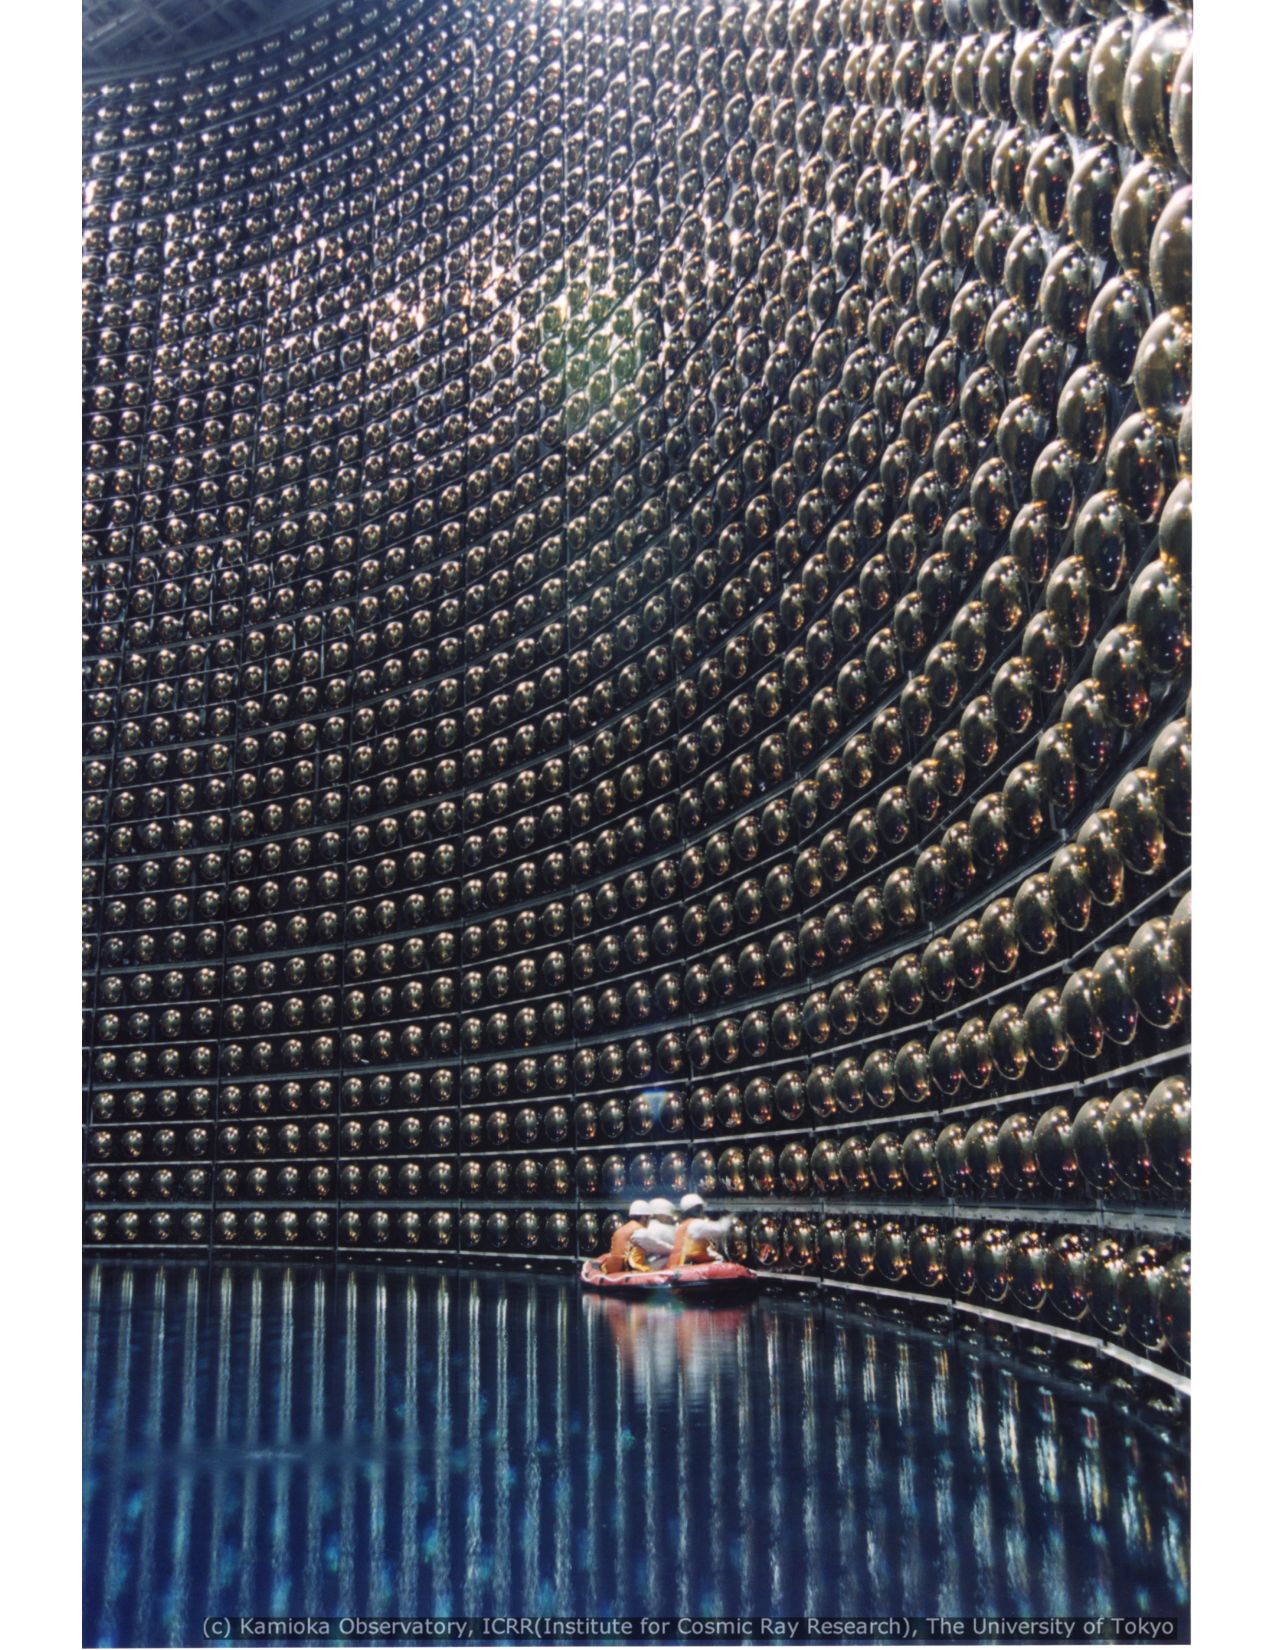
\includegraphics[scale=0.5]{Figures/superk.pdf}
		\caption[Inside Super-Kamiokande tank]{ {\textbf{Inside Super-Kamiokande tank}}\\Workers doing photomultipliers (PMTs) checking inside Super-Kamiokande detector \cite{superk_picture}.}
		\label{superk_picture}	
	\end{center}
\end{figure}

\section{Current Understanding of Neutrino Physics}
At this point, let me briefly summarize the understanding we currently have of neutrinos, obtained through the experiments and studies I mentioned above and many other experiments I left out from this historical overview. 

Neutrinos are chargeless leptons with small non-zero mass that only interact through the weak force. So far, we know of the existence of three types of them, that we call "flavor", and that are named after the charged lepton that accompanies them in charged-current weak interactions: electron neutrino ($\nu_e$), muon neutrino ($\nu_{\mu}$), and tau neutrino ($\nu_{\tau}$). 

Three bosons mediate the weak interaction: The $Z^{0}$, responsible for Neutral Current (NC) interactions; and the $W^{-}$ and $W^{+}$, responsible for Charged Current (CC) interactions, with both cases being represented by the Feynman diagrams in figure \ref{feymann_diag}. A CC neutrino-nucleus interaction changes the type of the quark it interacted with and produces its respective charged lepton, conserving lepton number and charge, i.e., an electron neutrino will always produce an electron. In NC neutrino-nucleus interactions, the incoming neutrino transfers momentum to the nucleus, with no charged lepton or hadron production.

\begin{figure}[h!]
	\begin{center}
		\includegraphics[scale=0.3]{Figures/feymann_diag.jpg}
		\caption[Feynman diagrams for the two types of weak interactions]{ {\textbf{Feymann Diagrams for the two types of weak interactions}} \\ On the left, the Feymman diagram for a Charged Current interaction, carried by a W boson. On the right, the Feymman diagram for a Neutral Current interaction, carried by a Z boson \cite{Lauren_thesis}.}
		\label{feymann_diag}	
	\end{center}
\end{figure}

We can observe different outcome products from neutrino interactions, depending on the energy of the incoming neutrino. At lower energies, $\lessapprox 10$ GeV, the dominant processes will be quasi-elastic scattering (QE), where neutrinos scatter off, and ejects out, a single nucleon. For interaction energies above 1232 MeV (the $\Delta$ baryon mass) resonance becomes energetically allowed, and this becomes the dominant process up to $4$ GeV. In it, neutrinos scatter off of a nucleon that gets excited. The deexcitation of the nucleon leads to a pion and a nucleon emission. From $4$ GeV beyond, the dominant process is Deep Inelastic Scattering (DIS), where neutrinos scatter directly off of nucleus' quarks, producing multiple hadrons in the final state. In figure \ref{nu_nucleus_int} you can see an illustration of each of these interactions and its final products. In figure \ref{nu_scatter}, you can see a summary of the existing measurements of CC neutrino cross-section divided by neutrino energy and plotted as a function of energy. 

\begin{figure}[h!]
	\begin{center}
		\includegraphics[scale=0.15]{Figures/neutrino_int_processes.jpeg}
		\caption[Neutrino-nucleus interactions and their products]{ {\textbf{Neutrino-nucleus interactions and their products}} \\ The left diagram shows a quasi-elastic scattering, ejecting a single nucleon. The middle diagram shows a resonant interaction, which produces a single pion and a nucleon. The right diagram shows a deep inelatic scattering, which produces multiple hadrons \cite{afro_phd}.}
		\label{nu_nucleus_int}	
	\end{center}
\end{figure}

\begin{figure}[h!]
	\begin{center}
		\includegraphics[scale=0.6]{Figures/nu_scatter_experiments.png}
		\caption[Total CC neutrino cross-section per nucleon as function of energy]{ {\textbf{Total CC neutrino cross-section per nucleon as function of energy}} \\ Summary of the existing measurements of CC neutrino-nucleon cross-section divided by neutrino energy and plotted as a function of energy. The QE is in red, the resonance in blue, the DIS in green, and the black is the total cross-section, when considering all the previous processes. It is shown which part of the energy spectrum can be explored by which experiment \cite{nu_scatter}.}
		\label{nu_scatter}	
	\end{center}
\end{figure}

\subsubsection{The CP Symmetry Violating Phase Parameter}

The $\delta$ parameter showed in the PMNS matrix in equation \ref{PMNS_factored} quantifies the charge conjugation and parity symmetry violation. The strong and electromagnetic interactions are invariant under CP symmetry, but some weak interaction processes are not. This violating phase parameter is also observed in the quark sector and was already measured. The CP symmetry violating phase parameter is still not observed in the lepton sector. 

The existence of CP symmetry violation is the hypothesis to explain why we have an asymmetry of matter and antimatter in the universe. We know the CP symmetry violation observed in the quark sector is not enough to explain it. Quantifying it in the lepton sector is essential to test this hypothesis \cite{cp_violation}. Among the current and future experiments aiming to measure the CP symmetry violating phase is the NuMI Off-axis $\nu_e$ Appearance (NO$\nu$A) \cite{NOVA}, the Tokai to Kamioka (T2K) \cite{T2K}, and the Deep Underground Neutrino Experiment (DUNE) \cite{dune_snowmass_22}, to name a few.

\subsubsection{The Character of the Neutrino Mass Spectrum (Mass Hierarchy)}

The equation \ref{nu_oscillation_final} limits that the data of neutrino oscillation experiments can only measure the mass-squared differences. Due to the tremendous growth of the neutrino experiment efforts in the past two decades, it is known that \cite{delta_2_1, delta_3_2}

\begin{equation}
	\Delta m^2_{21} = (7.53 \pm 0.18) \times 10^{-5} \ \text{eV}^2
	\label{delta_21}
\end{equation}

and 

\begin{equation}
	\Delta m^2_{32} = (2.34 \pm 0.09) \times 10^{-3} \ \text{eV}^2
	\label{delta_32_normal}
\end{equation}

or 

\begin{equation}
	\Delta m^2_{32} = (-2.37^{+0.07}_{-0.11}) \times 10^{-3} \ \text{eV}^2.
	\label{delta_32_inverted}
\end{equation}

The relative ordering $m_1 < m_2$ is known through observations of solar neutrinos, which are subject to resonant matter effects in the sun \cite{delta_2_1}. The value in Equation \ref{delta_32_normal} corresponds to what is called Normal Hierarchy and in Equation \ref{delta_32_inverted} to what is called Inverted Hierarchy. Normal hierarchy is the condition where the $m_1 < m_2 < m_3$. Inverted hierarchy is the condition where the $m_3 < m_1 < m_2$. You may find a schematic of the normal and inverted hierarchies in figure \ref{mass_hierarchy}. The precision of neutrino sector measurements has reached a point where the unknown hierarchy is a major hurdle to further progress \cite{prospects_patterson}.

\begin{figure}
	\begin{center}
		\includegraphics[scale=0.5]{Figures/mass_hierarchy.pdf}
		\caption[The Mass Hierarchy]{ {\textbf{The Mass Hierarchy}}\\The two possible neutrino mass hierarchies. The colors represent the approximate flavor admixtures present in each mass eigenstate \cite{prospects_patterson}.}
		\label{mass_hierarchy}	
	\end{center}
\end{figure}

\subsubsection{The $\mathbf{\theta_{23}}$ Octant Definition Problem}

The $\theta_{23}$ parameter is present is both $P_{\nu_\mu \rightarrow \nu_\mu}$ and $P_{\nu_\mu \rightarrow \nu_e}$ calculations. Most of the past neutrino experiments take advantage of an approximation that considers the existence of only two neutrino flavors due to limitations in their resolution. In this approximation the oscillation probabilities take the form of

\begin{equation}
	P_{\nu_\mu \rightarrow \nu_e} \propto \text{sin}^2(2\theta_{23}) \ \text{ and } \ P_{\nu_\mu \rightarrow \nu_\mu} \propto \text{sin}^2(2\theta_{23}),
	\nonumber
\end{equation}

which implies a redundancy in the value of $\theta_{23}$, with the possibilities being either $\theta_{23} > \pi/4$ or $\theta_{23} < \pi/4$. 
In more recent results, experiments such as NO$\nu$A, Main Injector Neutrino Oscillation Search (MINOS), and T2K, do not use this approximation, resulting in a 2-fold degeneracy solution for the mixing angle $\theta_{23}$. The latest results were presented by the NO$\nu$A Collaboration and can be seen in figure \ref{nova_result}, which shows the two best-fit values with their 90\% confidence level contours. In this study, NO$\nu$A Collaboration disfavored the maximal mixing ($sin^2 \theta_{23} = 0.5$) scenario with $2.6 \sigma$ significance \cite{NOVA}.

\begin{figure}
	\begin{center}
		\includegraphics[scale=0.7]{Figures/nova_result.pdf}
		\caption[Preliminary $\theta_{23}$ results from the NO$\nu$A Experiment]{ {\textbf{Preliminary $\theta_{23}$ results from the NO$\nu$A Experiment}} \\ Best fit (black dots) and allowed $90\%$ confidence level regions (solid black curves) of $\sin^2 \theta_{23}$ and $\Delta m^2_{23}$ for the normal hierarchy. The dashed curves show MINOS \cite{MINOS} and T2K \cite{T2K} $90\%$ confidence level contours \cite{NOVA}.}
		\label{nova_result}	
	\end{center}
\end{figure} 

\subsubsection{Short Baseline Neutrino Anomalies}

Over the past few decades, some neutrino experiments found inconsistencies between their expected un-oscillated neutrino flux at low energies and their measurements. Allow me to describe a few of them briefly. The Liquid Scintillator Neutrino Detector (LSND) at the Los Alamos Neutron Science Center published a paper in 2001 where they found an excess of electron-like antineutrino events in a primarily $\bar{\nu}_{\mu}$ beam \cite{lsnd}. Years later, the Mini Booster Neutrino Experiment (MiniBooNE) probed the same $L/E_{\nu}$ region and also found an excess of electron-like neutrino and antineutrino events in a primarily $\nu_{\mu}$ and $\bar{\nu}_{\mu}$ respectively, depending of the polarity of the Booster Neutrino Beam (BNB). Due to limitations on MiniBooNE's detector technology to separate electron and photon showers, their analysis was inconclusive as to whether the excess was due to new physics or background mis-modeling \cite{miniboone}. To address this issue, a new detector with better technology for particle identification was placed near MiniBooNE. This new experiment, named Micro Booster Neutrino Experiment (MicroBooNE), published its results in 2021. In this new report, they did not find an excess of electron-like neutrino events, but could not refute MiniBooNE's excess either \cite{microboone_lee}. 

The favorite hypothesis for new physics that could explain these anomalies is that a fourth neutrino would exist, called sterile neutrino ($\nu_s$). This neutrino, unlike the others, would not interact through any forces of the standard model (therefore ``sterile") and would only be indirectly observed whenever oscillating from or to one of the other flavors, which would justify those observations \cite{Lauren_thesis}. 
The short baseline neutrino anomalies and the existence of $\nu_s$s remain open questions in the field. 

\subsubsection{Majorana or Dirac Particles?}

In 1957, Goldhaber, Grodzins, and Sunya ran an experiment at the Brooke Haven National Laboratory to determine neutrinos' helicity. Helicity is a quantity in physics that encompasses the relative orientations of spin and linear momentum. If the projection of the spin onto the direction of momentum is a positive number, we call the particle ``right-handed". If the projection of the spin onto the direction of momentum is a negative number, we call the particle ``left-handed".
The results of the experiment, reported in the paper \cite{helicity}, indicated that all neutrinos are left-handed and all antineutrinos are right-handed. So far, we haven't had any evidence of left-handed antineutrinos or right-handed neutrinos. 
If neutrinos and antineutrinos and inherently different particles, like Goldhaber's \textit{et al.} experiment suggest, they are called ``Dirac particles". 
However, since neutrinos have mass, the helicity may be dependent on the reference frame in which the particle is observed. Theoretically, it is always possible to move to a reference frame in which the helicity would be flipped, and it is possible that neutrinos and antineutrinos are the same particles, just with different helicity. If that is the case, and neutrinos and antineutrinos are the same particles, they are called ``Majorana" particles. 
We currently have several experiments exploring this question, such as The Enriched Xenon Observatory (EXO) experiment \cite{exo}, KamLAND-Zen \cite{KamLAND-Zen}, and The GERmanium Detector Array (GERDA) \cite{gerda}. 


\chapter{Liquid Argon Time Projection Chambers in Neutrino Physics}

\label{Chapter:2}

\section{LArTPCs in Neutrino Physics}
Among a wide variety of detector technologies, liquid argon time projection chambers (LArTPCs) present a set of characteristics particularly interesting to neutrino physics. 
In a more general form, time projection chambers were first proposed by Nygren in 1974 \cite{Nygren}. They consist of a volume filled with a sensitive gas or liquid in a strong electrical field. When a charged particle passes through the active volume of the detector, the material is ionized, leaving a trail of ionization electrons. In the presence of an electric field, this ionization charge drifts towards charge sensitive electronics.
In the case of LArTPCs, the charge sensitive electronics consist of a set of at least two wire planes. In the first few planes, the passing of the ionization electrons through the wires produces an induction signal. In the last set of wires, the electrons are captured, producing a current, as shown in figure \ref{lartpc}. Combining information from the sets of wires and using a light trigger to calculate the drift time of the electrons in the event, it is possible to have a three dimensional calorimetric reconstruction of the track, as shown in figure \ref{lartpc_readout}. Alternatively, some experiments use the beam clock as trigger, without any light collection system. 
%
\begin{figure}[h!]
	\begin{center}
		\includegraphics[scale=0.12]{Figures/LARTPC.jpg}
		\caption[LArTPC]{ {\textbf{Liquid Argon Time Projection Chamber}} \\ liquid argon time projection chambers. When a particle passes through its fiducial volume and interacts with the liquid argon, ionization electrons and scintillation light are produced. The electric field drifts the electrons from where they are produced towards the planes of wires (right corner in the figure). Both charge and light produced are read by precision wires and a light collection system (in the figure, the orange bodies behind the wires), respectively.}
		\label{lartpc}	
	\end{center}
\end{figure}
%
\begin{figure}[h!]
	\begin{center}
		\includegraphics[scale=0.6]{Figures/Acciarri_fig2.pdf}
		\caption[LArTPC read out system]{ {\textbf{LArTPC read out system}} \\ Basic elements of the LArTPC read out system. It is needed a minimum of one induction wire plane, one collection wire plane and a light detection system. The information retrieved by those 3 components allow a 3D track reconstruction \cite{Acciarri_presentation}.}
		\label{lartpc_readout}	
	\end{center}
\end{figure}

\newpage
In 1977, not long after Nygren's proposal, Carlo Rubia noted that using liquid argon (LAr) as active material in a TPC was particularly advantageous for neutrino physics, since:
\begin{itemize}
	\item it is dense (1.4 g/cm$^3$), which increases the interaction probability;
 	\item it does not attach electrons, allowing long drift distances, which allows the construction of big detectors;
  	\item it has a high electron mobility;
   	\item argon is the third most abundant gas in the atmosphere, it is easy to obtain and purify, making it relatively cheap;
  	\item it is inert and and can be liquified with liquid nitrogen \cite{Rubia_ANewConcept}
\end{itemize}
Addicionaly, LAr is transparent to its own scintillation light. 
%
Most recently, LArTPCs have been the technology of choice of many neutrino physics experiments, such as Imaging Cosmic and Rare Underground Signals (ICARUS) \cite{ICARUS_proposal}, MicroBooNE \cite{microboone_proposal}, Short Baseline Neutrino Detector (SBND) \cite{SBND}, that together form the Short Baseline Neutrino (SBN) Program, and Deep Underground Neutrino Experiment (DUNE) \cite{dune_snowmass_22}, to name a few.
%
\section{The Short Baseline Neutrino Program}
%
In an attempt to investigate sterile neutrinos, Fermi National Laboratory (Fermilab) created the SBN Program. The program consists of three LArTPCs (SBND, MicroBooNE, and ICARUS) all located along the BNB beam. The principle is that, by having three different detectors of the same technology, exposed to the same beam, and all positioned at a short-baseline range, we will be able to more accurately constrain our flux of neutrinos and possibly investigate whether there are sterile neutrinos in the BNB beam oscilating to other flavors. Beyond that, it aims to study neutrino-nucleus scattering at the GeV energy scale and further develop LArTPC's construction and installation procedures \cite{SBN}.
%
Originally, ICARUS was, the first large-scale LArTPC to be used to further our understanding of neutrinos and was located underground at the The Gran Sasso National Laboratory and exposed to the CERN Neutrinos to Gran Sasso (CNGS) beamline \cite{ICARUS_proposal}. Most recently one of its modules, the T600, was refurbished, upgraded and has its new home at Fermilab, in the BNB beam. ICARUS T600 LArTPC is used as the far detector in the SBN Program. It is a $476$ton active mass LArTPC and it sits $600$ m from the target. 
%
\begin{figure}[h!]
	\begin{center}
		\includegraphics[scale=0.32]{Figures/SBN.png}
		\caption[The Short-Baseline Neutrino Program]{\textbf{The Short-Baseline Neutrino Program}\\The Short-Baseline Neutrino Program detectors as seen from an upper view at Fermilab. To the right is the neutrino beam target area where $8$ GeV protons from the Booster accelerator impinge a beryllium target. The beam is focused along the orange dashed line traveling toward the left (north). The SBND, MicroBooNE, and ICARUS \cite{SBN}.
		}
		\label{sbn_program}
	\end{center}
\end{figure}
%
The SBND is, as the name implies, the program's near detector and it consists of a $112$ton active mass LArTPC is at $110$ m from the target. It is currently under  installation phase and it is expected to be taking date mid-late next year,2023. In-between ICARUS and SBND, at $470$ m from the target, there is MicroBooNE, a $89$ton active volume LArTPC that has been taking da since 2015. Where each of the detectors are in the BNB beamline, at Fermilab, is illustrated in figure \ref{sbn_program}.
I will later describe in more details SBND and MicroBooNE, as they are the experiments in which I've carried my Ph.D. work. 
%
\section{The Deep Underground Neutrino Experiment}
%
The Deep Underground Neutrino Experiment (DUNE) is one of the most promising experiments for neutrino physics, as it aims to measure the CP violating phase in the leptonic sector, to determine the character of the neutrino mass spectrum, and to make precision measurements of oscillation parameters. Beyond the neutrino physics goals, DUNE also aims to search for baryon number violating processes and to perform precision measurements of neutrinos from a core-collapse supernova within the Galaxy, if one happens during the experiment's operating period. 
To accomplish such bold goals, DUNE designed with a near detector placed at Fermilab and a far detector at the Sanford Underground Research Laboratory in Lead, South Dakota. An intense neutrino beam of up to $2.4$ megawatts is produced at Fermilab, crosses the near detector, and travels $1,300$ kilometers downstream through Earth's crust to reach the far detector. In figure \ref{DUNE_full_schematic} you can see an schematic diagram of the experiment. 
%
\begin{figure}[h!]
	\begin{center}
		\includegraphics[scale=0.6]{Figures/DUNE_full_schematic.pdf}
		\caption[DUNE's full schematic]{ {\textbf{DUNE's full schematic.}} \\The figure shows the full DUNE's schematics, providing a view of the production of the neutrino beam, the Near Detector at Fermilab, the under crust travel of the beam, and the Far Detector at SURF \cite{dune_snowmass_22}.}
		\label{DUNE_full_schematic}	
	\end{center}
\end{figure}
%
DUNE's far detector is made of $4$ LArTPCs modules, of $10$ kton each. The near detector will have a combination of three different detection systems: a modular and optically segmented LArTPC of $\approx300$ tons (ND-LAr), a magnetized high-pressure Gas Argon Time Projection Chamber (GArTPC) surrounded by a calorimeterm (ND-GAr), a magnetized beam monitor consisting of an electromagnetic calorimeter, an inner target/tracker system and an active LAr target (SAND). \cite{dune_snowmass_22, dune_SAND}.

\chapter{The MicroBooNE Experiment}
The only supernova neutrinos detected to date was the SN1987A, from a supernova that happened at the Large Magellanic Cloud. A small amount of electron neutrinos from the event were observed at Kamiokande-II ($12 \nu_e$s), IMB ($8 \nu_e$s), and Baksan ($5 \nu_e$s). Despite the small dataset, a rich amount of analysis was published using the data, \cite{Kamiokande-II-PRL, Kamiokande-II-PRD, IMB, Baksan}. 
 On the occasion of a core-collapse supernova in our galaxy, measuring the flux of neutrinos and antineutrinos from all flavors will significantly enlighten the fields of astrophysics and neutrino physics. Therefore, one of DUNE's goals is to be prepared for such an event, as it is the most potent detector to measure the electron neutrinos signal from a supernova, \cite{dune_SAND}.
 In this chapter, I will explain the basics of supernovas and the neutrinos produced at them, why DUNE is particularly suitable to measure those neutrinos, and how using muos that decay at rest ($\mu$DARs) at the NuMI beam and interact in the MicroBooNE detector can help us improve neutrino-nucleus theoretical models and MeV-scale detection techniques in LArTPCs, which will be essential to accomplish the supernova detection in DUNE. 

\section{Core-Collapse Supernova Neutrino Detection in DUNE}
\subsubsection{Supernovas}
Supernova is the name given to the explosive chain of events that happens during the death of some stars. Particularly, core-collapse supernovas produce a massive number of neutrinos and antineutrinos whose spectrum, if measured, can inform on characteristics of the explosion. 
At the end of the life of a star that has $8-40$ solar masses, its body is made of concentric shells that were formed at each of its previous burning phases, them being: hydrogen, helium, carbon, neon, oxygen, and silicon, enveloping a core of nickel and iron. During its life, the stability of the star is a balance between the thermal pressure produced in the fusion process, which pulls everything in the outer direction, and its gravity pulling inward. When the mass of the iron core reaches $1.4$ solar masses, the pressure is not enough to balance the gravity, and the core starts to be compressed by the outer layers. Temperature and density in the core rise and the reaction

\begin{equation}
    e^{-} + p \longrightarrow n + \nu_e
\end{equation}

starts to happen more frequently, causing the pressure from electrons to lower even more and the star to collapse more rapidly. At the latest stages of the collapse, the density is such that even neutrinos get trapped in the core. Eventually, the pressure created by the nucleons degeneracy interrupts the collapse. The sudden stop of the collapse in the core causes a shock wave through the outer layers, and the star explodes. At the early stage of the shock wave, the density lowers, and the neutrinos manage to scape, creating an intense few-millisecond pulse called neutronization burst. 
After the neutronization burst, outer layers of the star still falling innard manage to stall the shock wave briefly. This stage is called the accretion phase. We still don't understand why the shock wave regains energy enough to proceed. One hypothesis is that neutrino reactions produce sufficient heat for the thermal pressure to give continuity to the explosion. 
Next, in the cooling phase, the star's energy is given away in many different processes that create neutrinos and antineutrinos of various flavors. A few of them are:

\begin{align}
    & \text{{\color{gray} electron pair annihilation:}}
    && e^{-} + e^{+} \longrightarrow \nu + \bar{\nu}, \\
    & \text{{\color{gray}electron-electron neutrino bremsstrahlung:}}
    && e^{\pm} + e^{\pm} \longrightarrow e^{\pm} + e^{\pm} + \nu + \bar{\nu} \\
    & \text{{\color{gray}electron-nucleon neutrino bremsstrahlung:}}
    && e^{\pm} + N \longrightarrow e^{\pm} + N + \nu + \bar{\nu} \\
    & \text{{\color{gray}photoannihilation:}}
    && \gamma + e^{\pm} \longrightarrow e^{\pm} + N + \nu + \bar{\nu} \\
    & \text{{\color{gray}nuclear de-excitation by neutrino pair production:}} 
    && ^{Z}_{A}X^{*} \longrightarrow ^{Z}_{A}X + \nu + \bar{\nu}
\end{align}

Given the wide variety of processes, measuring the flux of neutrinos and antineutrinos from all flavors is fundamental to help us better understand aspects of the supernova and what role the processes that happen during the explosion play in its development, \cite{Gardiner_thesis}. 

\subsubsection{Supernova detection in DUNE}

We have in operation or planned for the future a number of large detectors that would be able to detect signals from a core-collapse supernova that happens in our galaxy. The active material of those detectors are all water Cherenkov or hydrocarbon scintillator, making them mainly sensitive to electron antineutrinos, via inverse beta decay (the reaction in equation \ref{inverse_beta_decay_eq}). 
Therefore, relying solely on those detectors would preclude the measurement of the supernova eletron neutrino flux, which is by far the biggest component produced during the supernova's neutronization phase. 

Luckily, DUNE's active material is liquid argon, which is mainly sensitive to eletron neutrinos, via charged current scattering in $^{40}$Ar, as in:

\begin{equation}
    \nu_e + ^{40}Ar \longrightarrow ^{40}K + e^{-}
\end{equation}
    

\section{$\mu$ Decay At Rest ($\mu$DAR)-LAr Physics}
\section{Simulation of $\mu$DAR Events in MicroBooNE}
\subsection{NuMI Beamline Simulation}
\subsection{GENIE and MARLEY}
\section{Reconstruction of $\mu$DAR Events in MicroBooNE}


\section{Monte Carlo-Data Agreement}
\section{Background Assessment}
\section{Data Analysis}
\section{Conclusion}

\chapter{$\mu$ Decay At Rest $\nu_{e}$ Search in MicroBooNE}
The only supernova neutrinos detected to date was the SN1987A, from a supernova that happened at the Large Magellanic Cloud. A small amount of electron neutrinos from the event were observed at Kamiokande-II ($12 \nu_e$s), IMB ($8 \nu_e$s), and Baksan ($5 \nu_e$s). Despite the small dataset, a rich amount of analysis was published using the data, \cite{Kamiokande-II-PRL, Kamiokande-II-PRD, IMB, Baksan}. 
 On the occasion of a core-collapse supernova in our galaxy, measuring the flux of neutrinos and antineutrinos from all flavors will significantly enlighten the fields of astrophysics and neutrino physics. Therefore, one of DUNE's goals is to be prepared for such an event, as it is the most potent detector to measure the electron neutrinos signal from a supernova, \cite{dune_SAND}.
 In this chapter, I will explain the basics of supernovas and the neutrinos produced at them, why DUNE is particularly suitable to measure those neutrinos, and how using muos that decay at rest ($\mu$DARs) at the NuMI beam and interact in the MicroBooNE detector can help us improve neutrino-nucleus theoretical models and MeV-scale detection techniques in LArTPCs, which will be essential to accomplish the supernova detection in DUNE. 

\section{Core-Collapse Supernova Neutrino Detection in DUNE}
\subsubsection{Supernovas}
Supernova is the name given to the explosive chain of events that happens during the death of some stars. Mainly, core-collapse supernovas produce a massive number of neutrinos and antineutrinos whose spectrum, if measured, can inform the characteristics of the explosion. 
At the end of the life of a star that has $8-40$ solar masses, its body is made of concentric shells that were formed at each of its previous burning phases, them being: hydrogen, helium, carbon, neon, oxygen, silicon, enveloping a core of nickel and iron. During its life, the stability of the star is a balance between the thermal pressure produced in the fusion process, which pulls everything in the outer direction, and its gravity pulling inward. When the mass of the iron core reaches $1.4$ solar masses, the pressure is not enough to balance the gravity, and the core starts to be compressed by the outer layers. Temperature and density in the core rise and the reaction

\begin{equation}
    e^{-} + p \longrightarrow n + \nu_e
\end{equation}

starts to happen more frequently, causing the pressure from electrons to lower even more and the star to collapse more rapidly. At the latest stages of the collapse, the density is such that even neutrinos get trapped in the core. Eventually, the pressure created by the nucleons degeneracy interrupts the collapse. The sudden stop of the collapse in the core causes a shock wave through the outer layers, and the star explodes. At the early stage of the shock wave, the density lowers, and the neutrinos manage to escape, creating an intense few-millisecond pulse called neutronization burst. 
After the neutronization burst, outer layers of the star still falling innard manage to stall the shock wave briefly. This stage is called the accretion phase. We still don't understand why the shock wave regains energy enough to proceed. One hypothesis is that neutrino reactions produce sufficient heat for the thermal pressure to give continuity to the explosion. 
Next, in the cooling phase, the star's energy is given away in many different processes that create neutrinos and antineutrinos of various flavors. A few of them are:

\begin{align}
    & \text{{\color{gray} electron pair annihilation:}}
    && e^{-} + e^{+} \longrightarrow \nu + \bar{\nu}, \\
    & \text{{\color{gray}electron-electron neutrino bremsstrahlung:}}
    && e^{\pm} + e^{\pm} \longrightarrow e^{\pm} + e^{\pm} + \nu + \bar{\nu} \\
    & \text{{\color{gray}electron-nucleon neutrino bremsstrahlung:}}
    && e^{\pm} + N \longrightarrow e^{\pm} + N + \nu + \bar{\nu} \\
    & \text{{\color{gray}photoannihilation:}}
    && \gamma + e^{\pm} \longrightarrow e^{\pm} + N + \nu + \bar{\nu} \\
    & \text{{\color{gray}nuclear de-excitation by neutrino pair production:}} 
    && ^{Z}_{A}X^{*} \longrightarrow ^{Z}_{A}X + \nu + \bar{\nu}
\end{align}

Given the wide variety of processes, measuring the flux of neutrinos and antineutrinos from all flavors is fundamental to help us better understand aspects of the supernova and what role the processes during the explosion play in its development, \cite{Gardiner_thesis}. 

\subsubsection{Supernova detection in DUNE}

We have in operation or planned for the future a number of large detectors that would be able to detect signals from a core-collapse supernova that happens in our galaxy. The active material of those detectors is either water Cherenkov or hydrocarbon scintillator, making them mainly sensitive to electron antineutrinos via inverse beta decay (the reaction in equation \ref{inverse_beta_decay_eq}). 
Therefore, relying solely on those detectors would preclude the measurement of the supernova electron neutrino flux, which is the most significant component produced during the supernova's neutronization phase. 

Luckily, DUNE's active material is liquid argon, which is mainly sensitive to eletron neutrinos, via charged current scattering in $^{40}$Ar, as in:

\begin{equation}
    \nu_e + ^{40}Ar \longrightarrow ^{40}K + e^{-}
    \label{nu_scatter_eq}
\end{equation}
 
An example of a contribution to neutrino physics that a supernova neutrino detection could make in DUNE is to shine light into the mass hierarchy puzzle. Figure \ref{dune_supernova} shows how the time distribution of the incoming flux of the neutrinos of a $10$ kpc supernova in DUNE could depend on the mass hierarchy. In the case of inverted hierarchy, we should see an early excess of events from the neutronization phase, whether, in the case of normal hierarchy, we should see the absence of such events. The results from figure \ref{dune_supernova} are made assuming a model describer in reference \cite{dune_supernova_model}, but those results are assumed to be fairly model-independent \cite{kate_scholberg}. 

\begin{figure}[h!]
    \centering
    \includegraphics[width=150mm]{Figures/dune_supernova.jpeg}
    \caption[Predicted event time distribution for the detection of supernova neutrinos in a DUNE-like $40$ kt LArTPC]{{\textbf{Predicted event time distribution for the detection of supernova neutrinos in a DUNE-like 40 kt LArTPC}}\\ Predicted event time distribution for the detection of a $10$ kpc supernova neutrinos in a DUNE-like 40 kt LArTPC for each of the supernova stages. The blue curve assumes no oscillations, the green and the red curves assume oscillations for inverted and normal mass hierarchy, respectively \cite{kate_scholberg}.}Furthermore, being able to measure the flux of both neutrinos and antineutrinos is fundamental to further understanding exotic supernova processes \cite{Friedland}.
    \label{dune_supernova}
\end{figure}

Furthermore, being able to measure the flux of both neutrinos and antineutrinos is fundamental to further understanding exotic supernova processes \cite{Friedland}. 

\section{$\mu$ Decay At Rest $\nu_e$ Charged Current interactions in MicroBooNE}

\subsection{$\mu$ Decay At Rest in MicroBooNE}
As promising as the DUNE supernova neutrino program is, we currently lack an understanding of the MeV-scale neutrinos and LAr nucleus interactions, LArTPC reconstruction capabilities, and event identification at this energy range. 

As mentioned before, MicroBooNE is exposed to the BNB and NuMI beamlines. When on FHC mode, both beamlines produce a copious amount of antimuons that will, when decaying at rest, produce a muon antineutrino, an electron neutrino, and a positron, as shown in equation \ref{mudar_decay_eq}. The energy spectrum of the electron neutrinos from this decay is well-known and can be seen in picture \ref{mudar_nue_energy}. In figures \ref{numi_nue_flux} and \ref{numi_nu_flux} you can see the NuMI flux prediction of $\nu_e$s in MicroBoone by parents and the NuMI flux prediction in MicroBooNE of all neutrinos, respectively. 

\begin{equation}
	\mu^{+} \longrightarrow e^{+} + \nu_e + \bar{\nu}_{\mu}
    \label{mudar_decay_eq}
\end{equation}

\begin{figure}[h!]
    \centering
    \includegraphics[width=110mm]{Figures/mudar_nue_energy.jpg}
    \caption[Neutrino spectra of pion and muon decay at rest]{{\textbf{Neutrino spectra of pion and muon decay at rest}}\\ The red line is the energy of muon neutrinos from pion decay at rest, which is well-defined. The blue and the black lines refer to the energy spectrum of electron neutrinos and muon antineutrinos from positive muon decay at rest, respectively \cite{Yang2012}.}
    \label{mudar_nue_energy}
\end{figure}

Due to the nature of the decay, the electron neutrino will have kinetic energy $0 \leqslant KE_{\nu_e} \leqslant 52.8$ MeV, which overlaps nicely with the energy range of the supernova electron neutrinos we aim to detect in DUNE!

\begin{figure}[h!]
    \centering
    \includegraphics[width=180mm]{Figures/numi_nue_flux.jpeg}
    \caption[NumI $\nu_e$ flux in MicroBooNE]{{\textbf{NumI $\nu_e$ flux in MicroBooNE}}\\ On the right, the FHC $\nu_e$ neutrino flux at MicroBooNE from NuMI broken down by parent. Although a 60 MeV threshold is included in the percentages, the absolute value clearly shows the dominance of muon decays. On the left, the FHC neutrino flux is broken down by parent for each neutrino flavor. The percentages shown do not include an integration threshold on the angle. Decays from pions and muons dominate the majority of the flux across all angles \cite{krish_phd}.}
    \label{numi_nue_flux}
\end{figure}

\begin{figure}[h!]
    \centering
    \includegraphics[width=130mm]{Figures/numi_nu_flux.jpeg}
    \caption[NumI $\nu$ flux in MicroBooNE]{{\textbf{NumI $\nu$ flux in MicroBooNE}}\\ The flux prediction for all neutrino flavours in the FHC mode in neutrino angle. No integration threshold is applied in the percentages, and the electron neutrino flux percentage is boosted by muon decay at rest. The large angular spread in the flux is due to the positioning of MicroBooNE with respect to the NuMI beamline. The flux peaks at the target location and tails off further into the beamline. From angles above $20$ deg (midway into the decay pipe), the flux remains flat up to the absorber, where there is a large peak in the flux spectrum $\approx 120$ deg. After this, the flux is attenuated rapidly going into the muon-shield $ \ge 120$ deg.\cite{krish_phd}.}
    \label{numi_nu_flux}
\end{figure}
\newpage

\subsection{MeV-scale $\nu_e$-LAr Charged Current Interactions}

As explicitly shown in the \ref{nu_scatter_eq}, when MeV-scale neutrinos scatter in $^{40}$Ar, we have as product a $^{40}\textrm{K}^{*}$ and a $e^{-}$. From now on, I will refer to this electron as the ``main" electron of the signal. The energy of the incoming neutrino can be reconstructed as:

\begin{equation}
    E_{\nu} = E_e + \Delta_{final-initial} + T_{recoil} 
    \label{E_mudar_nu}
\end{equation}

where $E_e$ is the total energy of the outcoming electron and $T_{recoil}$ is the kinetic energy of the recoiling nucleon (which is negligible). As for $\Delta_{final-initial}$: 

 \begin{equation}
    \Delta_{final-initial} \equiv m_{final} - m_{initial}  
    \label{delta_fi}
\end{equation}

where $m_initial$ is the mass of the initial $^{40}$Ar nucleus, and $m_{final}$ is the mass state of the $^{40}\textrm{K}^{*}$ nucleus. The potassium nucleus can be at different excited states, depending on the event. Therefore, $m_{final}$ can be further described as:

\begin{equation}
    m_{final} = m_{final, g.s.} + E_x
    \label{mfinal}
\end{equation}

where $m_{final, g.s.}$ is the ground-state mass of a $^40$K nucleus and $E_x$ is the excitation energy. To reconstruct the total energy from the incoming neutrino, we need to look into the products from the de-excitation of the excited potassium nucleus, which are most commonly photons. Those photons can be indirectly measured in LArTPCs as they scatter on Ar atomic electrons, and the value of $\Delta_{final-initial}$ is given by:

\begin{equation}
    \Delta_{final-initial} = m_{g.s. \rightarrow g.s.} + \sum_{j}E_{\gamma, j}   
    \label{delta_fi_2}
\end{equation}

where $E_{\gamma,j}$ is the energy of each of the photons emitted and $m_{g.s. \rightarrow g.s.}$ is the mass difference between the ground state of the $^{40}$K nucleus and the ground state of the $^{40}$Ar nucleus, which is $1.5044$ MeV. 
It is also possible, although less likely, to have the excitation energy of the $^{40}$K high enough such that the de-excitation proceeds with the emission of a nucleon. A few of these channels still leave the daughter nucleus in an excited state, and there is an additional $\gamma$-ray or nucleon emission. This cascade continues until the daughter nucleus reaches the ground state. A diagram representing the different de-excitation channels can be seen in figure \ref{40K_deexcite}

\begin{figure}[h!]
    \centering
    \includegraphics[width=135mm]{Figures/40K_deexcitation.jpeg}
    \caption[De-excitation channels from an excited $^{40}$K nucleus, product of a CC MeV-scale $\nu_e$-LAr scattering]{{\textbf{De-excitation channels from an excited $^{40}$K nucleus, product of a CC MeV-scale $\nu_e$-LAr scattering}}\\  The excited $^{40}$K nucleus can reach its ground state by emitting $\gamma$-ray(s) (middle diagram), a neutron (diagram on the left), or a proton (diagram on the right). In case the emission of a nucleon still leaves the daughter nucleus in an excited state, more photons are emitted until the ground state is reached \cite{Gardiner_thesis}.}
    \label{40K_deexcite}
\end{figure}

The complexity of nuclear structures and the possible final state topologies for those interactions add challenges to the proper energy reconstruction of the supernova neutrino events. Therefore, it is fundamental that we take the opportunity presented by $\mu$DAR $\nu_e$s in MicroBooNE to study these interactions to improve our techniques. 


\section{Simulation of $\mu$DAR Events in MicroBooNE}

To properly evaluate the $mu$DAR events in MicroBooNE, we count with a chain of different simulation softwares to mimic the particle production and interactions at each step of the way. The chain is as it follows: First, we use the NuMI beamline simulation to to simulate the flux of neutrinos from the NuMI in MicroBooNE, this flux prediction is then handed to GENIE, a neutrino event generator, that propagates the neutrino into MicroBooNE. Then, another neutrino generator software, MARLEY, simulates the $mu$DAR $\nu_e$-LAr interaction, returnes the output to GENIE, that passes the result down to GEANT4, to do the detector simulation. I will go over each of those steps and the reasons why they are organized like this int his Chapter.

\subsection{NuMI Beamline Simulation}

NuMi >> BNB because addresses the 50 MeV threshold bla bla bla

\subsection{GENIE and MARLEY}

WHAT GENIE DOES AND HOW IT FAILS (fermi gas, does not have nuclear structures-----> need something better that has nuclear shell model), AND HOW MARLEY SAVES THE DAY 



\section{Reconstruction of $\mu$DAR Events in MicroBooNE}

\section{Monte Carlo-Data Agreement}

energy plots
position plots







\section{Background Assessment}
\section{Data Analysis}
\section{Conclusion}

%\chapter{Short Baseline Neutrino Detector's (SBND) Anode Plane Assemblies (APA) Assembly and Installation}
%
This work represents the first attempt to measure MeV-scale neutrino interactions in a LArTPC and extract a cross-section. Those measurements would be invaluable to the MeV-scale programs, nuclear physics models, and Supernova detection programs. 
However, the results were dominated by cosmic ray backgrounds and beam backgrounds. 

Looking  forward, several approaches can be taken to improve this analysis greatly, and I will list them below. 
\begin{enumerate}
 \item The blip reconstruction tools are under development and improving fast, but it was used in this work in one of its first versions. Therefore, it is a matter of time until the blip reconstruction group can turn the blip identification and reconstruction more efficient. Blip reconstruction could also benefit from a complete merge with the Pandora reconstruction tools if one would like to explore other methods of data selection and background identification.

 \item The analysis is dominated by cosmic ray background. MicroBooNE has a Cosmic Ray Tagger (CRT), composed of scintillator paddles on the top and bottom of the detector that could be used to identify cosmic rays entering the detector. The CRT data is currently being validated and processed in MicroBooNE, and soon it will be available and this analysis can benefit from it. This would help us remove full cosmic ray tracks and some bremsstrahlung and delta rays from them. However, it is unlikely we will be able to completely remove bremsstrahlung and delta rays without agressively reducing the fiducial volume.
 
 \item The other two background components in this analysis are activity from interactions of $\nu_{\mu}$s and $\nu_{e}$s from the beam. Muon's lifetime is $2.2$ $\mu s$, which means that we could reprocess the data through the steps presented in session $4.4$ to acquire information a few microseconds after the beam window, in which case the beam background would be non-existent for that portion of data. The impacts of it in the analysis is uncertain, and the resources cost of it would be significant, therefore more discussions on it with the MicroBooNE collaboration is needed. 
 
 \item The electron energy reconstruction currently assumes a flat energy deposition of $2$ MeV/cm. A more accurate energy deposition measurement could be obtained by using the ESTAR program. The ESTAR is a program that "calculates stopping power, density effect parameters, range, and radiation yield tables for electrons in various materials" \cite{ESTAR}. It has been used in LArTPCs before in ArgoNeut and MicroBooNE, but it is not yet deployed in the blip reconstruction tools used in this analysis \cite{argoneut_mev}, \cite{microboone_mev}. Implementing this tool would improve the signal energy reconstruction, but whether it would help with a better signal-background separation in uncertain. 
 
 \item This analysis could also benefit from lowering the hit threshold requirements on the hit finder tools. This would allow us to identify less energetic activity, which would be interesting for a second generation of this analysis, in which the deexcitation photons are included in the signal. Christopher Hilgenberg is currently wokring on lowering the hit threshold requirements in MicroBooNE. 
 
 \item Lastly, a next step for this work would be to fully evaluate the systematic uncertainties for this measurement. MicroBooNE has software structures in place to evaluate the flux systematics, GENIE systematics, and the detector systematics. However, one would have to work on the systematics from the MARLEY model. 
\end{enumerate}


%//\chapter{Novel LAr Purity Monitor Using Paul Traps}
%The SBND is another LArTPC detector part of the Short-Baseline Neutrino Program, together with MicroBooNE and ICARUS-T$600$. It is currently under construction and will consist of a $112$-ton LArTPC located at the BNB beamline. The diagram view of the SBN program detectors and their respective positions in the BNB beamline is shown in figure \ref{fig:sbn}.

\begin{figure}[h!]
    \centering
    \includegraphics[width=115mm]{Figures/sbn.jpg}
    \caption{Diagram view of the SBN program at Fermilab \cite{SBN}.}
    \label{fig:sbn}
\end{figure}

This LArTPC in particular is made of two different drift regions of $2$ m, with a central cathode, and two wire readout planes. A diagram of SBND and pictures of its anode planes are shown in picture \ref{fig:sbnd}. 

\begin{figure}[h!]
    \centering
    \includegraphics[width=110mm]{Figures/sbnd.jpg}
    \caption{Diagram view of the SBND detector on the left and pictures of SBND's anode wire planes on the right \cite{SBN}.}
    \label{fig:sbnd}
\end{figure}

The frame structures that you can see in the top left of figure \ref{fig:sbnd} are called Anode Plane Assemblies (APA). SBND has two of these frames. For each of them, half of the structure was made by our group and the other half was made by the Manchester group. We have a total of four structures, two made by our group and two made by the Manchester group, that in the end  form two APAs, one that is placed at the West side and another at the East side of the detector. 

\section{TPC Assembly and Installation}

After unboxing the APA structures, other members of the SBND assembly crew and I moved each of them to a clean tent where there is an alignment table. You can see the pictures of the tent and the APAs placed on the alignment table on picture \ref{fig:eastAPA}.

\begin{figure}[ht!]
    \centering
    \begin{subfigure}[t]{0.5\textwidth}
        \includegraphics[width=\textwidth]{Figures/eastAPA_post.jpg}
        \caption{}
    \end{subfigure}
    \hfill
    \begin{subfigure}[t]{0.49\textwidth}
        \includegraphics[width=\textwidth]{Figures/east_APA_pre.jpg}
        \caption{}
    \end{subfigure}
    \caption{On the left, a picture of the on-site crew that were working on moving the East APA to the alignment table. In it, you can see a half of an APA resting on the crib before its placement on the alignment table. On the right, a half of an APA recently placed on the alignment table.}
    \label{fig:eastAPA}
\end{figure}

 We then placed the two halves of the APA (one assembled by the SU team and another by the Manchester team) at each side of the table. We tested if the wires kept their nominal mechanical tensions and are still electrically conducting. Next, we aligned each frame and attached them, both mechanically and electrically, to form one bigger APA structure. On picture \ref{fig:aligment} you can see us working with Fermilab's alignment team on the East APA alignment. 

 \begin{figure}[h!]
    \centering
    \includegraphics[width=80mm]{Figures/IMG_3794.jpeg}
    \caption{SBND's team working with Fermilab's alignment team on the East APA alignment.}
    \label{fig:aligment}
\end{figure}

Next, the APA is carefully taken from the clean tent where we performed all the tests and placed in still final place in an structure called the Assembly Transport Frame (ATF), that supports the individual components of the TPC in place. We repeated all the procedures for the West APA.
\begin{figure}[ht!]
    \centering
    \begin{subfigure}[t]{0.46\textwidth}
        \includegraphics[width=\textwidth]{Figures/west_APA_pre.jpg}
        \caption{}
    \end{subfigure}
    \hfill
    \begin{subfigure}[t]{0.49\textwidth}
        \includegraphics[width=\textwidth]{Figures/westAPA_post.jpg}
        \caption{}
    \end{subfigure}
    \caption{On the left, a picture of me during and the West APA during the moving to its final place in the TPC. You can see the APA frame hanging by the crane during the operation. On the right, the on-site crew in front of the newly-installed West APA in the TPC.}
    \label{fig:westAPA}
\end{figure}

After both APAs were installed in the ATF and aligment adjusted, we started the field cage installation. The field cage are metal structures responsible to guarantee the shape and the uniformity of the electric field. In SBND, we have 8 field cage modules in each side of the detector, bottom, top, North, and South. You can see some pictures of the field cage installation in \ref{field_cage}

\begin{figure}[ht!]
    \centering
    \begin{subfigure}[t]{0.48\textwidth}
        \includegraphics[width=\textwidth]{Figures/field_cage_1.jpeg}
        \caption{}
    \end{subfigure}
    \hfill
    \begin{subfigure}[t]{0.48\textwidth}
        \includegraphics[width=\textwidth]{Figures/field_cage_2.jpeg}
        \caption{}
    \end{subfigure}
	\caption{On the left, a picture one of the top field cage modules being lowered to it place. Next to it, you can see another one already installed. At be back, you can see John Najdzion, the technician responsible for the installation procedures. On the right, you can see a pictur of the East side of the field cage with two top modules installed and one module of the North side installed.}
    \label{field_cage}
\end{figure}


% Apêndices
\appendix % Não deletar
\isappendixtrue % Não deletar
%\renewcommand\chaptername{Appendix}

%\chapter{An appendix title}
%\input{Appendices/A.tex}


%%%%%%%%%%%%%%%%%%%%%%%%%%%%%%%%%%%%%%%%%%%%%% EPÍLOGO %%%%%%%%%%%%%%%%%%%%%%%%%%%%%%%%%%%%%%%%%%%%
\bibliography{References}

\bibliographystyle{unsrt}

\begin{thebibliography}{10}

% Escreva um simples arquivo com referências ou insira  o .bbl
%1
\bibitem{griffiths} D. Griffiths, \textbf{Introduction to Elementary Particle Physics}. Second edition, Wiley-VCH Verlag GmbH \& Co. KGaA, Weinheim. ISBN 978-3-527-40601-2. 2008.

%2
\bibitem{nobel_leptons} K. V. L. Sarma, \textbf{Nobel Leptons}. arXiv:hep-ph/9512420. 1995.

%3
\bibitem{cowan_reines} C. L. Cowan, F. Reines, F. B. Harrison, H. W. Kruse, and A. D. McGuire. \textbf{Detection of the Free Neutrino: A Confirmation}. Science. 1956.

%4
\bibitem{Konopinski_Mahmoud} E. J. Konopinski, H. M. Mahmoud, \textbf{The Universal Fermi Interaction}. Phys. Rev. \textbf{92}. 1953.

%5
\bibitem{two_neutrinos} G. Danby, J-M. Gaillard, K. Goulianos, L. M . Lederman, N. Mistry, M. Schwartz, J. Steinberger, \textbf{Observation of high-energy neutrino reactions and the existence of two kinds of neutrinos}. Phys. Rev. Lett. \textbf{9}, 1, 36. 1962.

%6
\bibitem{the_story_of_the_neutrino} G. Rajasekaran, \textbf{The Story of the Neutrino}. arXiv:1606.08715. 2016.

%7
\bibitem{pontecorvo_1967} B. Pontecorvo, J. Exptl., \textbf{Neutrino Experiments and The Problem of Conservation of Leptonic Charge}. Theoret. Phys. \textbf{53}, 1717 (1967), Sov. Phys. JETP \textbf{26}, 984. 1968.

%8
\bibitem{MNS} Z. Maki \textbf{et al.}, \textbf{Remarks on the Unified Model of Elementary Particles}. Prog. Theor. Phys. \textbf{28}, 870-880. 1962.

%9
\bibitem{PMNS} B. Pontecorvo, \textbf{Inverse beta processes and nonconservation of lepton charge}. Soviet Phys. JETP. \textbf{7}, 172. 1958.

%10
\bibitem{Lauren_thesis} L. Yates, \textbf{Using the MicroBooNE Liquid Argon Detector
to Search for Electron Neutrino Interactions and Understand the MiniBooNE Anomaly}. FERMILAB-THESIS-2022-02. 2022.

%11
\bibitem{oscillation_math} C. Giunti, C. K. Kim, \textbf{Fundamentals of Neutrino Physics and Astrophysics}. Oxford University Press. ISBN 978-0-19-850871-7. 2007.

%12
\bibitem{first_kamioka_measure} Y. Fukuda \textit{et al.}, \textbf{Evidence for oscillation of atmospheric neutrinos}. Phys. Rev. Lett. \textbf{81}, 1562. 1998. 

%13
\bibitem{superk_picture} Workers doing PMTs checking during Super-Kamiokande's construction. Digital image. Super-Kamiokande collaboration, n.p. Web 17 May, 2010. 16 Jan 2017. \href{http://www-sk.icrr.u-tokyo.ac.jp/sk/gallery/index-e.html}{http://www-sk.icrr.u-tokyo.ac.jp/sk/gallery/index-e.html}

%14
\bibitem{afro_phd} A. Papadopoulou, \textbf{Lepton-Nucleus Scattering Measurements for Neutrino Interactions and Oscillations}. PhD thesis, MIT, 2022. 

%15
\bibitem{nu_scatter} S. Gollapinni1, \textbf{From eV to EeV: Neutrino Cross Sections across Energy Scales}. NuPhys 2015, Prospects in Neutrino Physics Barbican Center,UK. Proceedings at arXiv:1307.1341. 2016.

%16
\bibitem{cp_violation} S. Goswami  and N. Nath, \textbf{Determination of CP violation in the lepton sector}. AIP Conference Proceedings 2109, 110004. 2019.

%17
\bibitem{NOVA} P. Adamson \textit{et al.}, \textbf{Measurement of the neutrino mixing angle $\theta_{23}$ in NOvA}. arXiv:1701.05891. 2017.

%18
\bibitem{T2K} K. Abe \textit{et al.},\textbf{Measurements of neutrino oscillation in appearance and disappearance channels by the T2K experiment with $6.6 \times 10^{20} $ protons on target}. Phys. Rev. D \textbf{91}, 072010. 2015.

%19
\bibitem{dune_snowmass_22} A. Abed Abud \textit{et al.}, \textbf{Snowmass Neutrino Frontier: DUNE Physics Summary: Executive Summary of DUNE Physics Program}. arXiv:2203.06100. 2022.

%20
\bibitem{delta_2_1} A. Gando \textit{et al.}, \textbf{Neutrino Cross Section Future}. , 033001. 2013.

%21
\bibitem{delta_3_2} P. Adamson \textit{et al.}, \textbf{Combined Analysis of $\nu_\mu$ Disappearance and $\nu_\mu \rightarrow \nu_e$ Appearance in MINOS Using Accelerator and Atmospheric Neutrinos}. Phys. Rev. Lett. \textbf{112}, 191801 (2014); and update by A. Sousa for MINOS at XXVI International
Conference on Neutrino Physics and Astrophysics (Neutrino 2014), proceedings at arXiv:1502.07715. 2015.

%22
\bibitem{prospects_patterson} R. B. Patterson, \textbf{Prospects for measurement of the neutrino mass hierarchy}. arXiv:1506.07917v3. 2016.

%23
\bibitem{MINOS} P. Adamson \textit{et al.}, \textbf{Combined Analysis of $\nu_\mu$ Disappearance and $\nu_\mu$ $\rightarrow $ $\nu_e$ Appearance in MINOS Using Accelerator and Atmospheric Neutrinos}. Phys. Rev. Lett. \textbf{112}, 191801. 2014.

%24
\bibitem{lsnd} A. Aguilar-Arevalo et al. (LSND), \textbf{Evidence for neutrino oscillations from the observation of $\nu_e$ appearance in a $\nu_{\mu}$ beam}, Phys. Rev. D 64, 112007 (2001), arXiv:hep- ex/0104049.

%25
\bibitem{miniboone} M. Sorel \textit{et al.}, \textbf{MiniBooNE: first results on the muon-to-electron neutrino oscillation search}, J. Phys.: Conf. Ser. 110 082020, 2008.

%26
\bibitem{microboone_lee} P. Abratenko \textit{et al.}, \textbf{Search for an Excess of Electron Neutrino Interactions in MicroBooNE Using Multiple Final State Topologies}. arXiv:2110.14054. 2022.

\bibitem{helicity} M. Goldhaber \textit{et al.}, \textbf{Helicity of Neutrinos}. Phys. Rev. 109, 1015. 1958. 

\bibitem{exo} M. Auger \textit{et al.} (EXO Collaboration), \textbf{Search for Neutrinoless Double-Beta Decay in $^{136}$Xe with EXO-200}. Phys. Rev. Lett. 109 032505. arXiv:1205.5608. 2012.

\bibitem{KamLAND-Zen} S. Abe \textit{et al.} (KamLAND-Zen Collaboration), \textbf{First Search for the Majorana Nature of Neutrinos in the Inverted Mass Ordering Region with KamLAND-Zen}. arXiv:2203.02139. 2022

\bibitem{gerda} K.-H. Ackermann \textit{et al.} (GERDA Collaboration), \textbf{The GERDA experiment for the search of $0 \nu \beta \beta$ decay in $^{76}$Ge}. Eur. Phys. J. C 73 2330. arXiv:1212.4067. 2013.
%27
\bibitem{Nygren} D. R. Nygren, \textbf{The Time Projection Chamber: A New 4 pi Detector for Charged Particles}. eConf, vol. C740805, p. 58, 1974.

%28
\bibitem{Rubia_ANewConcept} C. Rubbia, \textbf{The Liquid Argon Time Projection Chamber: A New Concept for Neutrino Detectors}. 1977.

%29
\bibitem{Acciarri_presentation} R. Acciarri (LArIAT Collaboration), \textbf{LArIAT:
Liquid Argon In a Testbeam} Internal report. DocDB-1975.

%30
\bibitem{ICARUS_proposal} S. Amerio \textit{et al.}, (ICARUS Collaboration), \textbf{Design, construction and tests of the ICARUS T600 detector}. Nucl. Instr. and Meth. in Phys. Res. \textbf{A 527}, 329. 2004.

%31
\bibitem{microboone_proposal} H. Chen \textit{et al.}, \textbf{A Proposal for a New Experiment Using the Booster and NuMI Neutrino Beamlines: MicroBooNE}. 2007.

%32
\bibitem{SBND} \textbf{Short-Baseline Near Detector (SBND)}. n.d. Retrieved from \href{http://sbn-nd.fnal.gov}{http://sbn-nd.fnal.gov}

%33
\bibitem{SBN} P. Machado, O. Palamara, and D. Schmitz, \textbf{The Short-Baseline Neutrino Program at Fermilab}. arXiv:1903.04608. 2019. 

%34
\bibitem{dune_SAND} Matteo Vicenzi, for the DUNE collaboration, \textbf{SAND - System for on-Axis Neutrino Detection - in the DUNE Near Detector complex}. The 22nd International Workshop on Neutrinos from Accelerators (NuFact2021). Italy, 2021.
%35
\bibitem{microboone_electronics} R. Acciarri, \textit{et al.} \textbf{Noise Characterization and Filtering in the MicroBooNE Liquid Argon TPC}. JINST 12 P08003. 2017.

%36
\bibitem{microboone_design} R. Acciarri, \textit{et al.} \textbf{Design and construction of the MicroBooNE detector}. JINST 12 P02017. 2017. 

%37
\bibitem{lar_excimers} W. Pontseele. \textbf{Search for Electron Neutrino Anomalies with the MicroBooNE Detector}. PhD thesis, Oxford U., 2020.

%38
\bibitem{uboone_pmt} Microboone photomultiplier. \href{https://news.fnal.gov/2015/07/microboone- photomultiplier/}{https://news.fnal.gov/2015/07/microboone- photomultiplier/}.

%39
\bibitem{RFQ_website} J. Orwig, \textbf{Cockcroft-Walton's successor: a peep inside the new RFQ and how it works}. 2012. Retrieved from http://www.fnal.gov/pub/today/archive/archive\_2012/today12-11-02\_RFQReadmore.html

%40
\bibitem{LINAC_website} \textbf{Fermilab Linac}. Retrieved from \url{http://www-bd.fnal.gov/proton/linac.html/}

%41
\bibitem{booster_website} \textbf{Booster Department}. Retrieved from http://www-ad.fnal.gov/proton/booster.html

%42
\bibitem{paper_numibeamline} P. Adamson, \textit{et al.} (MINOS Collaboration) \textbf{The NuMI neutrino beam}. Nucl. Instr. Meth. A \textbf{806}, 279-306. 2016.

%43
\bibitem{numi} \textbf(Target Systems). Retrieved from \url{https://targets.fnal.gov/NuMI_neutrino_beam.html}

%44
\bibitem{krish_phd} K. Mistry, \textbf{First Measurement of the Flux-Averaged Differential Charged-Current Electron-Neutrino and Antineutrino Cross Section on Argon with the MicroBooNE Detector}. PhD thesis, U. of Manchester, 2021. 

%45
\bibitem{numi_redmine} MicroBooNE Collaboration, \textbf{NuMI Documentation}. Internal Documentation. Retrieved from \url{https://cdcvs.fnal.gov/redmine/projects/uboone- physics-analysis/wiki/NuMI_Documentation#Using- NuMI-samples-for-an-analyser}. 
%[1]
\bibitem{Kamiokande-II-PRL} S. Hirata, et al., Kamiokande-II Collaboration. \textbf{Observation of a neutrino burst from the supernova SN1987A}. Phys. Rev. Lett. \textbf{58}, 1490–1493. 1987.

%[2]
\bibitem{Kamiokande-II-PRD} S. Hirata, et al., Kamiokande-II Collaboration. \textbf{Observation in the Kamiokande-II detector of the neutrino burst from supernova SN1987A}. Phys. Rev. D \textbf{38}, 448–458. 1988.

%[3]
\bibitem{IMB} M. Bionta, et al., IMB Collaboration, \textbf{Observation of a neutrino burst in coincidence with supernova 1987A in the Large Magellanic Cloud}. Phys. Rev. Lett. \textbf{58}, 1494–1496. 1987. 

%[4]
\bibitem{Baksan} Alexeyev et al., \textbf{Detection of the neutrino signal from SN 1987A in the LMC using the INR Baksan underground scintillation telescope}. Phys. Lett. B \textbf{205}, 209–214. 1988.

%[5]
\bibitem{Supernova_Neutrino_Detection} K. Scholberg. \textbf{Supernova Neutrino Detection}. arXiv:1205.6003. 2012.

\bibitem{Gardiner_thesis} S. Gardiner. \textbf{Nuclear Effects in Neutrino Detection}. PhD thesis,  U. C. Davis, 2018.

%[6]
\bibitem{kate_scholberg} K. Scholberg. \textbf{Supernova signatures of neutrino mass ordering}. Journal of Physics G: Nuclear and Particle Physics 45, 014002. 2017.

%[7]
\bibitem{dune_supernova_model} L. Hudepohl et al. \textbf{Neutrino signal of electron-capture supernovae from core collapse to cooling}. Physical Review Letters 104, 251101. 2010.

%[8]
\bibitem{Friedland} A. Friedland. \textbf{SN signal modeling: collective effects} Talk presented at the May 2018 DUNE Collaboration Meeting, Batavia, Illinois. 2018. 

%[9]
\bibitem{Yang2012} Z. Yang \textit{et al.}. \textbf{Simulation study of neutrino nucleus cross section measurement in a segmented detector at a spallation neutron source}. Chinese Physics C. \textbf{36}. 538-543. 2012. 


%[10]
\bibitem{g4} S. Agostinelli \textit{et al.}, (Geant4 Collaboration). \textbf{Geant4—a simulation toolkit}. Nucl. Instrum. Meth. A 506, 250-303. 2003.

\bibitem{minerva} L. Aliaga \textit{et al.}, (MINER$\nu$A Collaboration). \textbf{Design, Calibration, and Performance of the MINERvA Detector}.  arXiv:1305.5199. 2013. 

\bibitem{minos} P. Adamson, \textit{et al.}, (MINOS Collaboration), \textbf{MINOS Technical Design Report}. NuMI-NOTE-GEN-0337. 1998.

%[11]
\bibitem{fluka} A. Ferrari \textit{et al.}, (FLUKA Collaboration). \textbf{Fluka:
a multi-particle transport code}. 2021. \href{http://www.fluka.org/content/manuals/FM.pdf
}{http://www.fluka.org/content/manuals/FM.pdf}

%[12]
\bibitem{ppfx} L. Aliaga Soplin. \textbf{Neutrino Flux Prediction for the NuMI Beamline} Ph.D. thesis, William-Mary Coll., 2016.

\bibitem{Walecka-Donnelly} J. S. O’Connell, T. W. Donnelly, and J. D. Walecka. \textbf{Semileptonic weak interactions with C12}. Physical Review C 6, 719-733. 1972.

\bibitem{noise_filter} R. Acciarri \textit{et al.} (MicroBooNE Collaboration). \textbf{Noise Characterization and Filtering in the MicroBooNE Liquid Argon TPC}. JINST 12, P08003. arXiv:1705.07341. 2017. 

\bibitem{avinay_thesis} A. Bhat. \textbf{MeV Scale Physics in MicroBooNE}. PhD thesis, Syracuse U., 2021.

\bibitem{pandora} R. Acciarri \textit{et al.} \textbf{The Pandora multi-algorithm approach to automated pattern recognition of cosmic-ray muon and neutrino events in the MicroBooNE detector}. Eur. Phys. J. C, 78. 2018.

\bibitem{signal_proc} C. Adams \textit{et al.}, (MicroBooNE Collaboration), \textbf{Ionization Electron Signal Processing in Single Phase LArTPCs. Part II. Data/Simulation Comparison and Performance in MicroBooNE}, JINST 13, P07007. 2018.

\bibitem{deexcitation-model} W. Hauser and H. Feshbach. \textbf{The inelastic scattering of neutrons}. Physical Review 87, 366. 1952.
 
\bibitem{will_CM_Aug} W. Foreman. \textbf{MeV-scale 'Blip' Reconstruction in MicroBooNE \&
Measuring the Ambient Radon Rate}. MicroBooNE Collaboration Meeting. Fermilab, August 2022. Internal document DocDB 38470. 2022. 

\bibitem{lariat_calorimetry_lar} W. Foreman, \textit{et al.}, (LArIAT Collaboration). \textbf{Calorimetry for low-energy electrons using charge and light in liquid argon}. arXiv:1909.07920. 2020.

\bibitem{BPULE} Y. Zhu. \textbf{Upper limit for Poisson variable incorporating systematic uncertainties by Bayesian approach}.

\bibitem{ESTAR}  M.J. Berger, \textit{et al.} \textbf{ESTAR, PSTAR, and ASTAR: Computer Programs for Calculating Stopping-Power and Range Tables for Electrons, Protons, and Helium Ions (version 1.2.3).}. Available at \href{http://physics.nist.gov/Star}{http://physics.nist.gov/Star}. 2005.

\bibitem{argoneut_mev} R. Acciarri, \textit{et al.}, (ArgoNeuT Collaboration). \textbf{Demonstration of MeV-Scale Physics in
Liquid Argon Time Projection Chambers Using ArgoNeuT.} FERMILAB-PUB-18-559-ND. arXiv:1810.06502. 2018.

\bibitem{microboone_mev} R. Acciarri \textit{et al.}, (MicroBooNE Collaboration). \textbf{MeV-scale Physics in MicroBooNE}. MICROBOONE-NOTE 1076-PUB. 

\end{thebibliography}

%%%%%%%%%%%%%%%%%%%%%%%%%%%%%%%%%%%%%%%% FIM DO DOCUMENTO %%%%%%%%%%%%%%%%%%%%%%%%%%%%%%%%%%%%%%%%%
\end{document}